
\section{Proofs}
\label{app:equiv_dist}

\subsection{Proofs for Equivariance of Gaussians [Proposition \ref{prop:equivnormal}]}

In this section, we prove that the Gaussian probability density function is $\SOtwo$-equivariant.

\begin{prop*}
 Given multivariate normal distribution $\mathcal{N}(\mu,\Sigma)$ over $\mathbb{R}^2$ with probability density function $p_{\mu, \Sigma}$ and $g\in \SOtwo$, then $p_{g\mu, g\Sigma g^T} (v) = p_{\mu, \Sigma} (g^{-1}v)$ for all $v \in \mathbb{R}^2$.
\end{prop*}

\begin{proof}
\begin{align*}
P_{g\mu, g\Sigma g^T}(v) &= \frac{1}{2 \pi \det{(g\Sigma g^T)}} \exp{(-\frac{1}{2}(v-g\mu)^T (g \Sigma g^T)^{-1} (v - g\mu))} \\
 &= \frac{1}{2\pi \det{(\Sigma})} \exp{(-\frac{1}{2}(g^{-1}v-\mu)^T g^T g^{-T} \Sigma^{-1} g^{-1} g (g^{-1}v -\mu))} \\
&= \frac{1}{2\pi \det{(\Sigma})} \exp{(-\frac{1}{2}(g^{-1}v-\mu)^T \Sigma^{-1} (g^{-1}v -\mu))}\\ 
&= P_{\mu, \Sigma}(g^{-1}v) 
\end{align*}
\end{proof}


\begin{prop*} 
Given a normal distribution $\mathcal{N}(\mu,\Sigma)$, its group-actioned $\mathcal{N}(g\mu, g\Sigma g^T)$ is also a valid normal distribution. 
\end{prop*}

\begin{proof}
We prove the proposition by proving that $g\Sigma g^T$ is a symmetric positive definite matrix.

1) \textit{(Symmetry)} $(g\Sigma g^T)^T = g^{TT} \Sigma^T g^T = g\Sigma g^T$.

2) \textit{(Positive Definite)}  Let $v\in \mathbb{R}^2 $ and $v\neq 0$. Let $w = g^T v$, note that $w\neq 0$. Then $v^T g\Sigma g^T v =  w^T \Sigma w >0$, which implies $\Sigma$ is a positive definite matrix.  
\end{proof}

\subsection{Equivariance of construct for positive definite and symmetric $\Sigma$ [Proposition \ref{prop:pds}]}

%We want a neural network $f$ such that $z \xrightarrow[]{f} \mu, \Sigma$. $\mu$ is a $\rho_1$ feature. 

Note that every positive definite symmetric matrix can be written as $\Sigma = MM^T$ for some $M\in GL_2(\mathbb{R})$, so we can represent $\Sigma$ by a map $\varphi$ where
\begin{align*}
       \varphi \colon \mathrm{GL}_2(\mathbb{R}) &\to \mathrm{PosDefSym}_2(\mathbb{R})  \\ 
    M &\mapsto M M^T
\end{align*}

\begin{prop*}
$\varphi$ is $\SOtwo$-equivariant.
\end{prop*}
\begin{proof}
$\varphi (gMg^T) = gMg^T (gMg^T)^T = gMg^T g^{TT} M^T g^T = gMM^Tg^t = g\varphi(M)g^T $
\end{proof}

We defined the one-sided inverse of $\varphi$ as $\psi$:
\begin{align*}
        \psi \colon \mathrm{PosDefSym}_2(\mathbb{R}) &\to \mathrm{GL}_2(\mathbb{R})    \\ 
        \Sigma &\mapsto Q \lambda^{\frac{1}{2}}
\end{align*}
where $Q\lambda Q^T$ is the eigendecomposition of $\Sigma$ and $Q$ is orthogonal.   That is, $\varphi (\psi(\Sigma)) = \Sigma$.
\begin{prop*}
$\psi$ is $\SOtwo$-equivariant.
\end{prop*}
\begin{proof}
For symmetric positive definite matrix $\Sigma$, its eigenvector $v_i$ and eigenvalue $\lambda_i$ follows the eigenequation
\[
    \Sigma v_i = \lambda_i v_i .
\]
For $\forall g \in \SOtwo$, 
\[
  g\Sigma v_i = \lambda_i g v_i \implies g\Sigma g^{-1} g v_i = \lambda_i g v_i \implies (g\Sigma g^{-1}) (g v_i) = \lambda_i (g v_i) ,
\]
so $gv_i$ is an eigenvector to $g\Sigma g^{-1}$, with corresponding eigenvalue $\lambda_i$.

Therefore, 
\[
\psi (g\Sigma) = gQ\Lambda^{\frac{1}{2}} = g\psi (\Sigma).
\]
\end{proof}

% \subsection{Equivariance for Quadratic Form}
% Two n-ary quadratic forms $\phi$ and $\psi$ over $\R$ are equivalent if there exists a nonsingular linear transformation $M \in GL(n)$ such that $\phi(x) = \psi (Mx), \forall x\in \R^n$. Under the equivalence $M$, the symmetric matrix $A$ of $\phi$ and the symmetric matrix $B$ of $\psi$ are related by a change of bases: $A = M^TBM$.

% \begin{prop*}
% Given $\SOtwo$-equivariant neural network $f_1:\R^2\rightarrow \R^2$ and $f_2:\R^2\rightarrow \R^2$, for all non-zero $\rho_1$ feature $h \in \R^2$, defining the linear transformation $M(h) = [f_1(h), f_2(h)]$, the symmetric matrix $\Sigma(h) = M(h)M(h)^T$ for the corresponding quadratic form is equivariant.
% \end{prop*}
% \begin{proof}
% \begin{align*}
%     C(gh) & = M(gh)M(gh)^T = 
%     \begin{bmatrix} f_1(gh) & f_2(gh)\end{bmatrix}
%     \begin{bmatrix} f_1(gh)^T \\ f_2(gh)^T\end{bmatrix} \\
%     & = \begin{bmatrix} gf_1(h) & gf_2(h)\end{bmatrix}
%     \begin{bmatrix} f_1(h)^Tg^T \\ f_2(h)^Tg^T\end{bmatrix} \\
%     & = g\begin{bmatrix} f_1(h) & f_2(h)\end{bmatrix}
%     \begin{bmatrix} f_1(h)^T \\ f_2(h)^T\end{bmatrix}g^T \\ 
%     & = gM(h)M(h)^Tg^T = g\Sigma(h)g^T
% \end{align*}
% \end{proof}

% Since the covariance matrix $\Sigma$ is a positive definite symmetric matrix, it defines a quadratic form over $\R$. For non-zero $\rho_1$ feature $h \in \R^2$, we can define $\Sigma(h) =  M(h)M(h)^T$. Then the defined quadratic form $x^T\Sigma x$ is equivalent to standard quadratic form $x^Tx$ under equivalence $M(h)$, and this equivalence is equivariant. In other words, the neural network changes the bases of identity matrix equivariantly for covariance matrix.



\subsection{Proof of Proposition \ref{prop:equivtoinvar}: The Equivariant Model Gives an Invariant Conditional Distribution. }


We now prove Proposition \ref{prop:equivtoinvar}.

\begin{prop*}[Proposition \ref{prop:equivtoinvar}]
If the one-step probabilistic forecasting model $f_\theta$ is $G$-equivariant, then the conditional probability distribution $p_\theta( \mathbf{x}_{t+1:t+k} | \mathbf{x}_{1:t}, \mathbf{e})$ is invariant as in \autoref{eqn:invariant_prob}.
\end{prop*}

\begin{proof}
Since $\mathbf{x}_{1:t}$ are known, we define $\Sigma_{1:t} = \epsilon \mathrm{Id}$ for $\epsilon$ small approximating a delta distribution at $\mu_{1:t} = \mathbf{x}_{1:t}$.
We then evaluate $\mu_{j+1},\Sigma_{j+1} = f_\theta(\mu_{j-t+1:j}, \Sigma_{j-t+1:j}, \mathbf{e})$ autoregressively for $j=1,\ldots,k$.  Finally define 
\begin{equation}
\begin{aligned}
    p_\theta( \mathbf{x}_{t+1:t+k} | \mathbf{x}_{1:t}, \mathbf{e}) &=
    \prod_{j=1}^k  p_\theta( \mathbf{x}_{t+j} | \mathbf{x}_{j:t+j-1}, \mathbf{e}) \\
    &= \prod_{j=1}^k p_{N(\mu_{t+j},\Sigma_{t+j})}(\mathbf{x}_{t+j}). 
\end{aligned}
\label{eq:timeseriespdf}
\end{equation}

For $g \in \SOtwo$, we want to show 
\[
    p_\theta( g\mathbf{x}_{t+1:t+k} | g\mathbf{x}_{1:t}, g\mathbf{e}) = p_\theta( \mathbf{x}_{t+1:t+k} | \mathbf{x}_{1:t}, \mathbf{e}).
\]
  Thus for $g\mathbf{x}_{1:t}, g\mathbf{e}$ we initialize $g \mu_{1:t},g\Sigma_{1:t}g^{T}$ since $g\Sigma_{1:t}g^T = gg^T\Sigma_{1:t}= \Sigma_{1:t}$. Applying $f_\theta$ repeatedly and invoking equivariance, we obtain 
\begin{align}
    g\mu_{t+j},g\Sigma_{t+j}g^{T} = f_\theta(g\mu_{j:t+j-1}, g\Sigma_{j:t+j-1}g^{T}, g\mathbf{e}). 
\end{align}
for $j =1,\ldots,k$.  Then by \autoref{eq:timeseriespdf}, 
\[
    p_\theta( g\mathbf{x}_{t+1:t+k} | g\mathbf{x}_{1:t}, g\mathbf{e}) =
    \prod_{j=1}^k p_{N(g\mu_{t+j},g\Sigma_{t+j}g^{T})}(g\mathbf{x}_{t+j}).
\]
Then by Proposition \ref{prop:equivnormal} this is 
\[
  \prod_{j=1}^k p_{N(\mu_{t+j},\Sigma_{t+j})}(g^{-1}g\mathbf{x}_{t+j}),
\]
which cancels $g^{-1}g = 1$, and applying \autoref{eq:timeseriespdf} again gives  $p_\theta( \mathbf{x}_{t+1:t+k} | \mathbf{x}_{1:t} \mathbf{e})$.  
\end{proof}



\subsection{Proof that MRS is a strictly proper scoring rule}
\label{app:properscoring}

Scoring rules are summary measures to evaluate probabilistic forecasts; they take in the forecasted distribution and the event or value that materializes and assign a numerical score. As defined in \cite{properscoring},  a scoring rule is proper if it is maximized when the forecaster recovers the ground truth distribution. It is strictly proper if the maximum is unique.

\begin{prop*} 
MRS is a strictly proper score.
\end{prop*}
\begin{proof}
%For arbitrary predictive distributions $P$ and $Q \in \mathbb{R}$, $MRS(P,Q) \geq 0$. Moreover, $MRS(P,Q) = 0$ holds if and only if $P=Q$.
For arbitrary function $h$, we first define the scoring rule
\[
 S(R;z) = -|R| + \frac{1}{\alpha}(|R| - |R(z)|)\mathbb{1}\{z\in R^C\} + h(z),
\]
which means if the forecaster quotes region $R$ at the level $\alpha\in (0,1)$ and $z$ materializes, then the score $S(R;z)$ will be rewarded, where $R$ and $R(z)$ are defined as ellipsoid parametric by $\mu$ and $\Sigma$. Then the expected score under the probability measure $P\in \mathcal{P}$ which $z$ follows is defined as
\[
 S(R;P) = \int S(R;z) \, dP(z). 
\]
For $P\in \mathcal{P}$, let $R_*$ denote the unique true $P$-region at level $\alpha$. We say that scoring rule $S$ is strictly proper if 
\[
 S(R_*;P) \geq S(R;P),
\]
for all region $R$ and for all probability measures $P\in \mathcal{P}$, where equality holds if and only if $R = R_*$. 

We identify $P$ with the associated distribution function so that $P(R_*^C)=\alpha$. If $R_* \subset R$, then
\begin{align*}
    S(R_*;P) - S(R;P) & = \int -|R_*| \, dP(z) + \frac{1}{\alpha} \int_{R_*^C} (|R_*| - |R(z)|) \, dP(z) \\
    & + \int |R| \, dP(z) - \frac{1}{\alpha} \int_{R^C} (|R| - |R(z)|) \, dP(z) \\
    & = -|R_*| + |R| + \frac{1}{\alpha}|R_*|P(R_*^C) - \frac{1}{\alpha}|R|P(R^C) - \frac{1}{\alpha}\int _{R_*^C \setminus R^C} |R(z)| \, dP(z) \\
    & \geq |R| - \frac{1}{\alpha}|R|P(R^C) - \frac{1}{\alpha}|R|(P(R_*^C)-P(R^C)) \\
    & = 0, 
\end{align*}
as it is supposed to be. If $R \subset R_*$, then an analogous argument applies. 

Putting $h(z) = 0$ and reversing the sign of the scoring rule, yields the negatively oriented regional score. Finally, the mean score of this oriented regional score is our MRS, which is then proved to be proper.
\end{proof}


\section{Supplementary: Equivariant Matrix Output Layer Construction}
\label{app:matrix}

Let 
\[
    \rho_1(\theta) = \begin{pmatrix}
    \cos{\theta} & -\sin{\theta} \\
    \sin{\theta} & \cos{\theta}
    \end{pmatrix} 
    \qquad\qquad
        M = \begin{pmatrix}
    a & b \\
    c & d
    \end{pmatrix}
\]
where $a,b,c,d$ are trainable parameters.
Consider input $f \colon S^1 \to \mathbb{R}$, then
\[
F(f) = \int_{\theta=0}^{2\pi} f(\theta) \rho_1(\theta) M \rho_1(-\theta) d\theta.
\]
Define $\rho_{reg}(\phi)(f)(\theta) = f(\theta-\phi)$.  
\vspace{5px}
\begin{prop*}
The convolution $F$ is equivariant, i.e.,
\[
F(\rho_{reg}(\phi) f) = \rho_1(\phi) F(f) \rho_1(-\phi).
\]
\end{prop*}
\begin{proof}
We compute
\begin{align*}
    F(\rho_{reg} (\phi)f) 
    &= \int_{\theta=0}^{2\pi}  \rho_{reg}(\phi)(f)(\theta) \rho_1(\theta) M\rho_1(-\theta) d \theta \\
    &= \int_{\theta=0}^{2\pi}  f(\theta-\phi) \rho_1(\theta) M\rho_1(-\theta) d \theta \\
    &= \int_{u=-\phi}^{2\pi-\phi} f(u) \rho_1(u+\phi)M\rho_1(-u-\phi)du \quad (\text{substituting } u = \theta - \phi) \\ 
% \end{align*}
% Since the integrand is periodic, this is equal to integrating from $u=0$ to $u = 2\pi,$ 
% \begin{align*}
    &= \rho_1(\phi) \cdot \left( \int_{u=-\phi}^{2\pi-\phi} f(u) \rho_1(u)M\rho_1(-u)du \right) \cdot \rho_1(-\phi) \\
    &=  \rho_1(\phi) F(f) \rho_1(-\phi). 
\end{align*} 
The last substitution follows from the fact the integrand is periodic of period $2\pi$. Since the integral is over the whole circle, this equal to taking the limits of integration to be $0$ and $2\pi$.
\end{proof}

\vspace{3px}

\paragraph{Discritization.}
If the function $f$ is discretized, such that $f_i = f(i2\pi/n)$.  Then the mapping $F$ is given by 
\[
F(f) = \sum_{i=0}^{n-1} f_i \rho_1(i2\pi/n) M \rho_1(-i2\pi/n).
\]

\paragraph{Compatibilitiy with matrix exponential}

For a $n \times n$ matrix $M$ define 
\[
\exp(M) = \sum_{k=0}^\infty M^k/k!.
\]
Matrix exponentiation is equivariant with respect to conjugation.  That is for $g \in \mathrm{GL}_n(\mathbb{R})$, 
\[
\exp(gMg^{-1}) = \sum_{k=0}^\infty (gMg^{-1})^k/k!. 
\]
Now note that
\[
(gMg^{-1})^k = (gMg^{-1}) (gMg^{-1}) \ldots (gMg^{-1}) = gMM \ldots Mg^{-1} = g M^k g^{-1}.
\]
So then 
\[
\sum_{k=0}^\infty (gMg^{-1})^k/k! = \sum_{k=0}^\infty gM^kg^{-1}/k! = g \left( \sum_{k=0}^\infty M^k/k! \right) g^{-1} = g \exp(M) g^{-1}.
\]

\paragraph{Structured Network Output}

So the last layers of the neural network will be $\exp \circ F$ which outputs an invertible $2 \times 2$ matrix and satisfies 
\[
(\exp \circ F)(\rho_{reg}(\phi) f) = \rho_1(\phi) (\exp \circ F)(f) \rho_1(-\phi).
\]


\section{Supplementary: Baseline Algorithms}

\subsection{Score Function for Probabilistic Forecast}
% \subsection{Problem Formulation}

We consider a probabilistic approach to trajectory forecasting. Ideally, we want the predicted distribution to be both sharp and valid under the definition in \Eqref{eq:coverage}. To quantify the uncertainty, we review the classic score function Mean Interval Score (MIS) and derive a 2 dimensional extension, Mean Regional Score (MRS).

% \leo{Is 'interval' a proper terminology here? Empirically it's a 1-d concept, for n-d interval people always mean region with square bounding. It's confusing especially when the mean interval score below is a 1-d metric.} 

% For each agent in the scene, we estimate a sequence of $k$ prediction regions $\Hat{C}_{t+1:t+k}$ for $\mathbf{x}_{t+1:t+k}$. The intervals $\Hat{C}$ are dependent on a significance level $\alpha$, denoted  as $\Hat{C}^{\alpha}$. 

% given by $p_\theta( \mathbf{x}_{t+1:t+k} | \mathbf{x}_{1:t}, \mathbf{e})$,


\paragraph{Mean Interval Score.}
Mean Interval Score (MIS) is a proper scoring rule \cite{properscoring} for interval forecasts that rewards narrower confidence intervals and encourages coverage. 
%
Specifically, let $Y  \sim {P}_Y$ be a one-dimensional random variable, and an upper bound $u$, a lower bound $l$ be its estimated $\frac{\alpha}{2}$ and $(1-\frac{\alpha}{2})$ quantiles respectively, MIS is defined using samples $y_i \sim {P}_Y$.
 %
\begin{align}
    \mathrm{MIS}(u,l; Y) = \frac{1}{N} \sum_{i=1}^{N}[(u-l) +
     \frac{2}{\alpha}(y_i-u)\mathbb{1}\{y_i>u\}\nonumber 
     + \frac{2}{\alpha}(l-y_i)\mathbb{1}\{y_i<l\} ] 
    \label{eq:mis}
\end{align}
%
Where the three terms in  \Eqref{eq:mis} accounts for the width of the interval, and how much the sample point exceeds the upper bound and the lower bound, respectively. MIS has the advantage of being easy to compute and does not require the model to be parametric \cite{properscoring}. It can also be used as an objective function for probabilistic forecasting \cite{wu2021quantifying}. 


\paragraph{Mean Regional Score.}
For n-D distributions, we introduce a new metric called the Mean Region Score (MRS), which generalizes MIS to higher dimensions. 
%
Let $Z \sim {P}_Z$ be an n-dimensional continuous random variable. First, we need to generalize  $\alpha$-quantile and define the  confidence region. Let the region bordering $z$ as $R(z)$, the  confidence region of level $\alpha$ 
\begin{align}
R_P(\alpha) =  \inf \lbrace R(z)  | \int_{R(z)} P( z ) dz \geq \alpha \rbrace
\end{align}
is the smallest region whose probability exceeds  level $\alpha$.

\begin{figure}
    \centering
  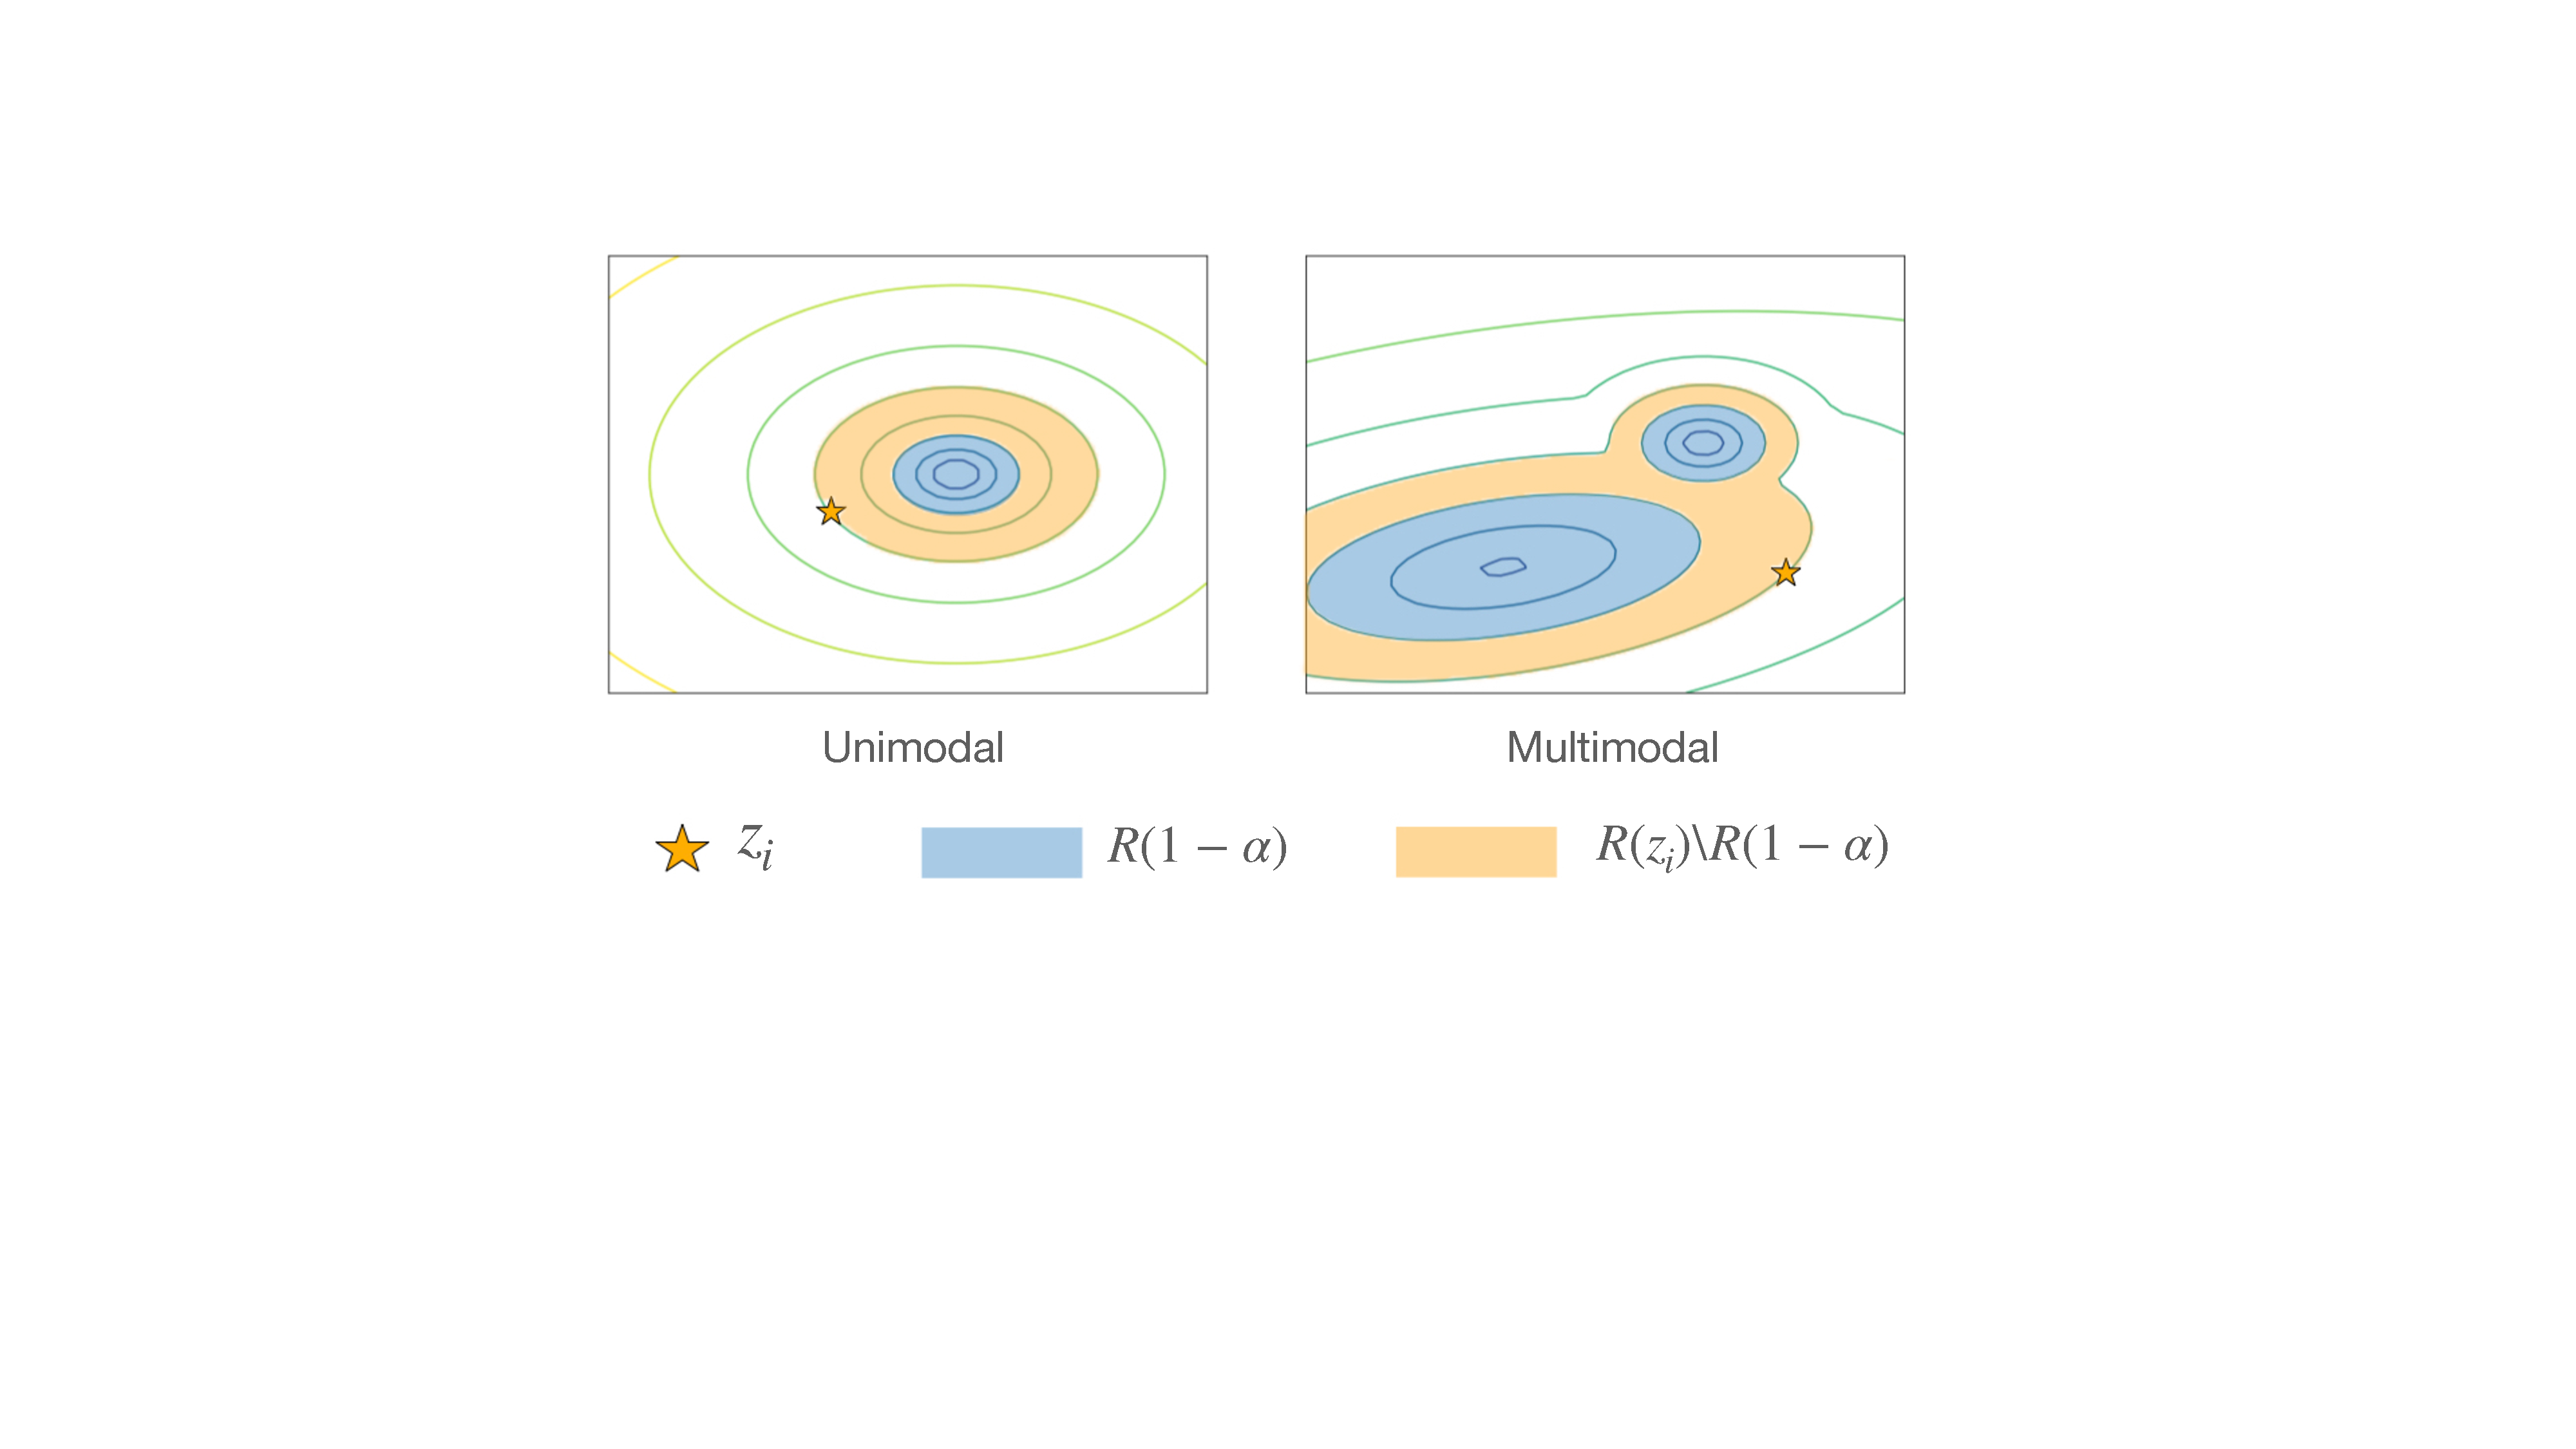
\includegraphics[width=.8\linewidth]{equivariance/figs/mrs.pdf}
  \caption{MRS illustration for   unimodal and multimodal distributions. Given a sample $z_i$, MRS  calculates the area of blue region plus that of the the orange region scaled by $1/\alpha$. }
  \label{fig:mrs}
\end{figure}
When the distribution is Gaussian $P_Z =\mathcal{N}(\mu, \Sigma)$ with mean $\mu \in \mathbb{R}^n$ and the covariance matrix $\Sigma \in \mathbb{R}^{2\times 2}$ that is positive definite. The $(1-\alpha)$ confidence region of an n-D multivariate normal distribution $P = \mathcal{N}(\mu, \Sigma)$ is an ellipsoid that can be written as \cite{slotani1964tolerance}:
\[
    R(1-\alpha) = \{ z| (z-\mu)^T \Sigma^{-1} (z-\mu) \leq  \chi_n^2(1-\alpha)\}.
\]
where $\chi_n^2$ is the chi-squared distribution with n degrees of freedom.
Then, for a given sample $z_i \in \mathbb{R}^n$, we can draw an ellipsoid whose edge coincides $z_i$ defined as 
\[
    R(z_i) = \{z|(z-\mu)^T\Sigma^{-1}(z-\mu) \leq c'\} 
\]
where $c' = (z_i - \mu)^T \Sigma^{-1} (z_i - \mu)$.


% The smallest confidence region of  $1-\alpha$ could be viewed as a superlevel set of points with probability greater than a threshold $\zeta_{1-\alpha}$. \cite{multimodalconfidence}




The MRS score of the $(1-\alpha)$ prediction interval thus can be evaluated as:
%
\begin{align}
    \mathrm{MRS}(R ;Z) = \frac{1}{N} \sum_{i=1}^N  [|R(1-\alpha)| +   \frac{1}{\alpha}| R(z_i) \backslash R(1-\alpha)| \mathbb{1} \{z_i \in R^C(1-\alpha)\}]
\label{eq:mrs}
\end{align}
where the first term  corresponds to the area of the confidence region and the second term measures how much each data $z_i$ deviates from the region. $|\cdot|$ measures the size of the set.  It is also easy to prove (see Appendix \ref{app:properscoring}) that MRS is a proper scoring rule \cite{properscoring}, which means MRS is optimized if and only if the distribution $P$ recovers that of $Z$.

Figure \ref{fig:mrs} illustrates MRS for both unimodal and multimodal distributions.  Note that when the distribution is single-modal, the confidence interval in \Eqref{eq:mrs} is both \textit{equally tailed} and the \textit{shortest} confidence interval. For  multi-modal distributions,  we solve for the \textit{smallest} confidence region to cover probable events. In appendix \ref{app:mrsgeneral} we present a method to estimate MRS for arbitrary 2-D distributions, where we divide the domain space into small grids to estimate density, and obtain $R(1-\alpha)$ and $R(z_i)$ by assembling high density regions.
%


%For an arbitrary distribution $P$ over $\mathbb{R}^2$, we can define the confidence region $S_P$ as the superlevel set $S_P(1-\alpha) = \lbrace x \in \mathbb{R}^2 | p(x) \geq c(\alpha) \rbrace$, where $c(\alpha)$ is defined such that 

\subsection{Empirical method for estimating MRS for general 2D distribution }
\label{app:mrsgeneral}

We present an empirical method to estimate MRS given any 2D distribution. We first discretize the 2D space that is the domain of the probability distribution into $n$ grid cells, indexing them as $g_i$ where $i\in \{1,\ldots,j\}$. Then we can numerically estimate the density of each grid cell $p(g_i)$ for $i= 1,\ldots,n$. The confidence region can be estimated by selecting the grid cells with the highest likelihoods until they sum to $1-\alpha$. 
\[
R(1-\alpha) = \bigcup_{i\in K} g_i, \quad K =  \text{argmin}_K: \Sigma_{i\in K} p(g_i) \geq 1-\alpha
\]
where $K$ is the superlevel set of grid cells $g_i$ whose empirical probability density is at least  $1-\alpha$.

Similarly, we define the estimated region 
\[ 
R (z_i) = \bigcup g_i \quad \text{ for } p(g_i) \geq p(z_i)
\]
as the superlevel set of data point $z_i$. This way, we can calculate MRS for any 2D using the estimated $R(1-\alpha)$ and $R(z_i)$ in the MRS formula. 
\[
    \mathrm{MRS}(R ;Z) = \frac{1}{N} \sum_{i=1}^N  [|R(1-\alpha)| +     \frac{1}{\alpha}| R(z_i) \backslash R(1-\alpha)| \mathbb{1} \{z_i \in R^C(1-\alpha)\}]
\]

Figure \ref{fig:empiricalmrs} illustrates the idea, this method is used to estimate the MRS scores for multimodal methods \texttt{Trajectron++} and \texttt{MFP} in our experiments.

\begin{figure}[!h]
  \centering
  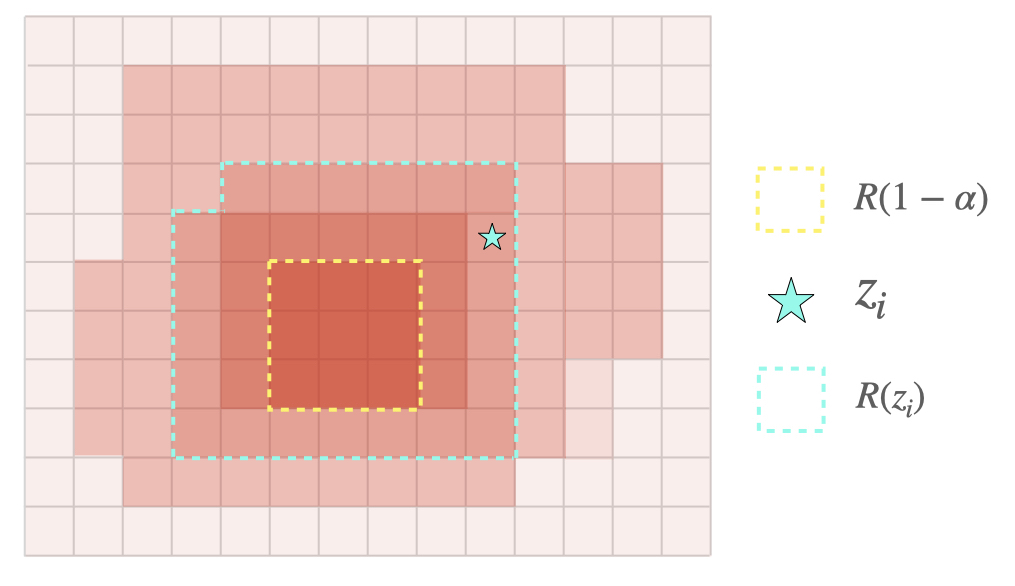
\includegraphics[width=.5\linewidth]{equivariance/figs/empmrs.jpeg}
  \caption{Illustration for empirical MRS estimation, where we calculate the probability density at each grid, and select the highest density grids to construct $R(z_i)$ and $R(1-\alpha)$. This way, we may approximate MRS numerically.}
  \label{fig:empiricalmrs}
\end{figure}


\subsection{Conformal algorithm for 2-D Time Series}
\label{app:conformal}
We extend the inductive conformal prediction (ICP) algorithm \cite{shafer2008tutorial} to conformally estimate a confidence region for 2D forecasts. Given an exchangeable set of trajectory observations $\mathcal{D} = \{ (\mathbf{x}_{1:t}^{(i)}, \mathbf{e}^{(i)}), \mathbf{x}_{t+1:t+k}^{(i)}\}_{i=1}^l$ and a new sample $(\mathbf{x}_{1:t}^{(l+1)}, \mathbf{e}^{(l+1)})$, the ICP algorithm returns $k$ prediction intervals,$[\Gamma^{\alpha}_1, \ldots, \Gamma^{\alpha}_k]$, one for each timestep, such that:
\[
\mathbb{P}[\: \forall j \in \{1,\ldots, k\}, \: x_{t+j} \in \Gamma^{\alpha}_j(\mathbf{x}^{(l+1)})\: ] \geq 1-\alpha
\]
for any underlying predictive model. This inequality is the \textit{validity} condition. \cite{2021conformal} proves the 1-D case for time-series forecasting validity; we leave proving it for the 2-D case for future work.

ICP requires an underlying forecasting model and a choice of nonconformity score. In our case, LSTM and ECCO are both models that take as input $(\mathbf{x}_{1:t}, \mathbf{e})$ and outputs $\mathbf{x}_{t+1:t+k}$. We select root mean square error (RMSE) as our nonconformity score as it is commonly used in the 1-d setting and naturally extends to high dimensions. We split the training set into the proper training set and a calibration set of equal size: $\mathcal{D} =\mathcal{D}_{train} \bigcup \mathcal{D}_{cal}$. We train our model $M$ on $\mathcal{D}_{train}$ and obtain the critical nonconformity scores $\hat{\gamma_1}, \ldots, \hat{\gamma_k}$ as in algorithm 1 in \cite{2021conformal}.
%\autoref{alg:conformal}.
Then, for input $(\mathbf{x}_{1:t}, \mathbf{e})$ and $ \hat{x}_{t+1:t+k} = M(\mathbf{x}_{1:t}, \mathbf{e})$ we can construct a set of confidence intervals 

\[
\Gamma^{\alpha}_j(\mathbf{x}^{(l+1)}_{(1:t)}) = \{ x\in \mathbb{R}^2 \; | \; RMSE(x, \hat{x}_j) \leq \hat{\gamma}_j\} \; \text{ for } j \in\{1,\ldots, k\} 
\]

We illustrate some example scenes with confidence regions provided by conformal-ECCO in figure \ref{fig:conformal}. Note that the regions for timestep $j$ are given by $\hat{\gamma}_j$, hence are the same for every scenario. With our choice of RMSE as the nonconformity score, the region is a circle; they appear elliptical due to scale compression. 
\begin{figure*}[ht]
    \centering
    \begin{subfigure}[b]{0.245\linewidth}
        \centering
        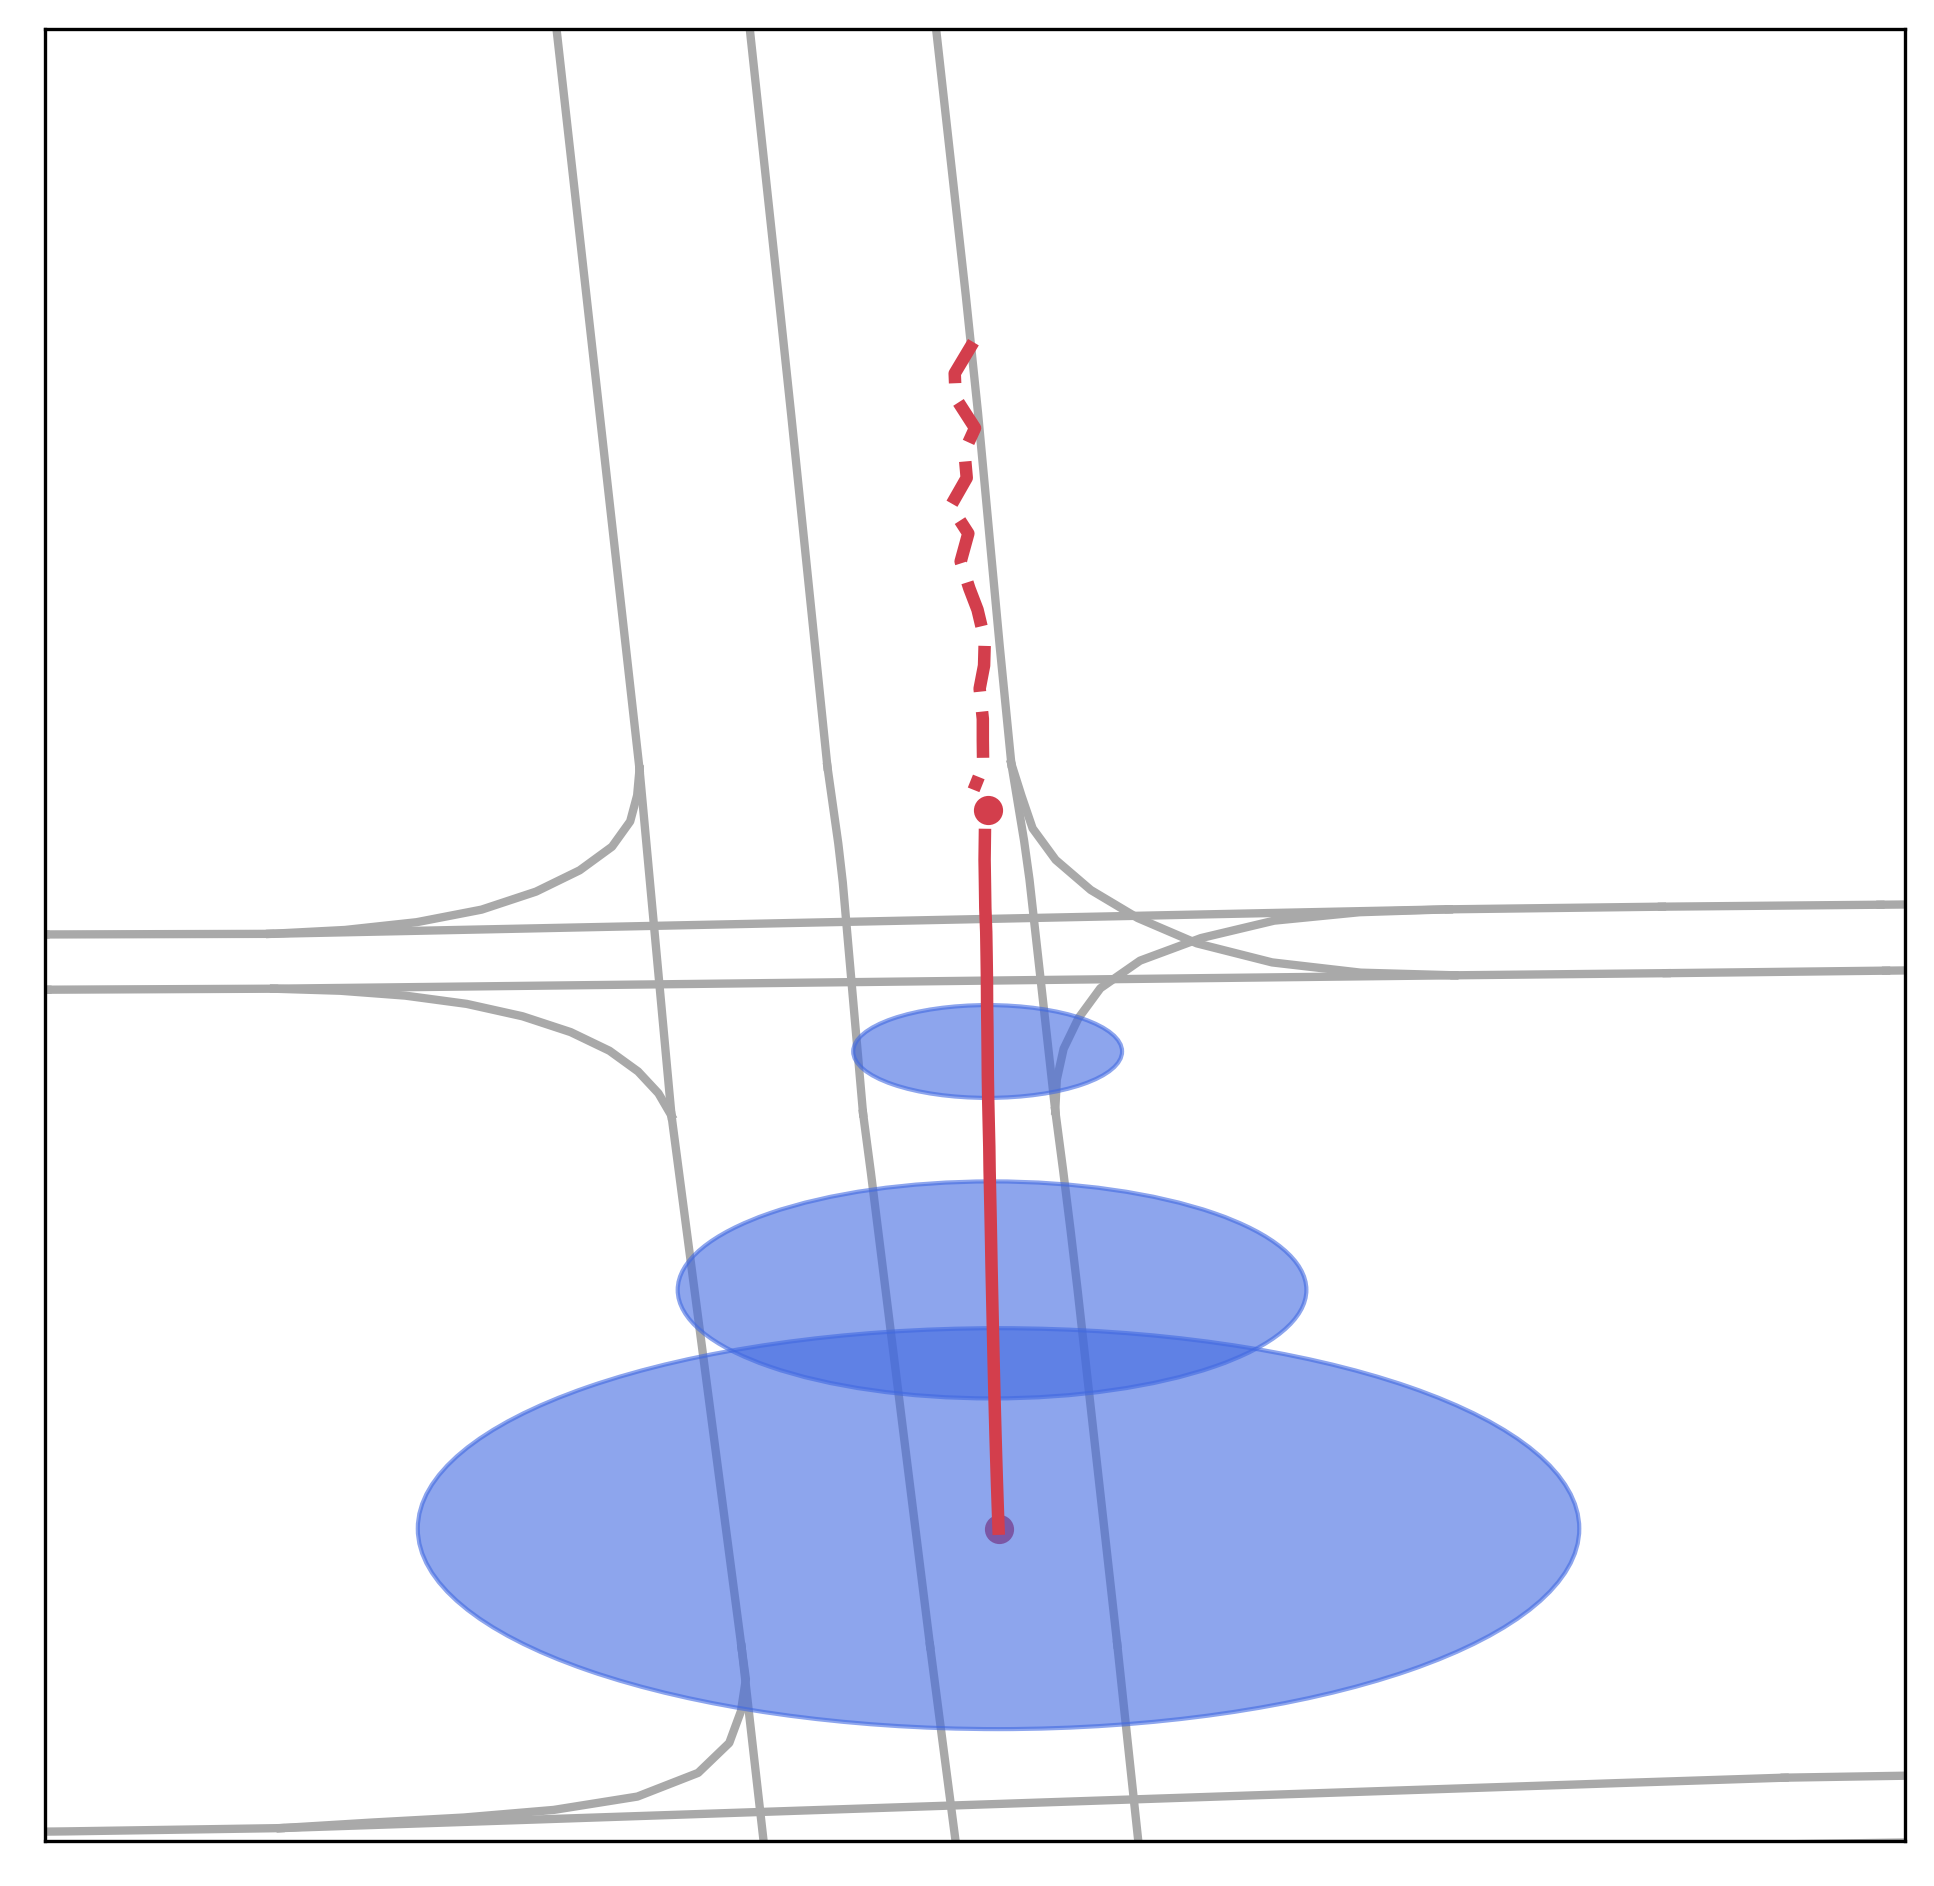
\includegraphics[width=\linewidth]{equivariance/figs/conf1.png}
        \caption{}
    \end{subfigure}%
    \begin{subfigure}[b]{0.245\linewidth}
        \centering
        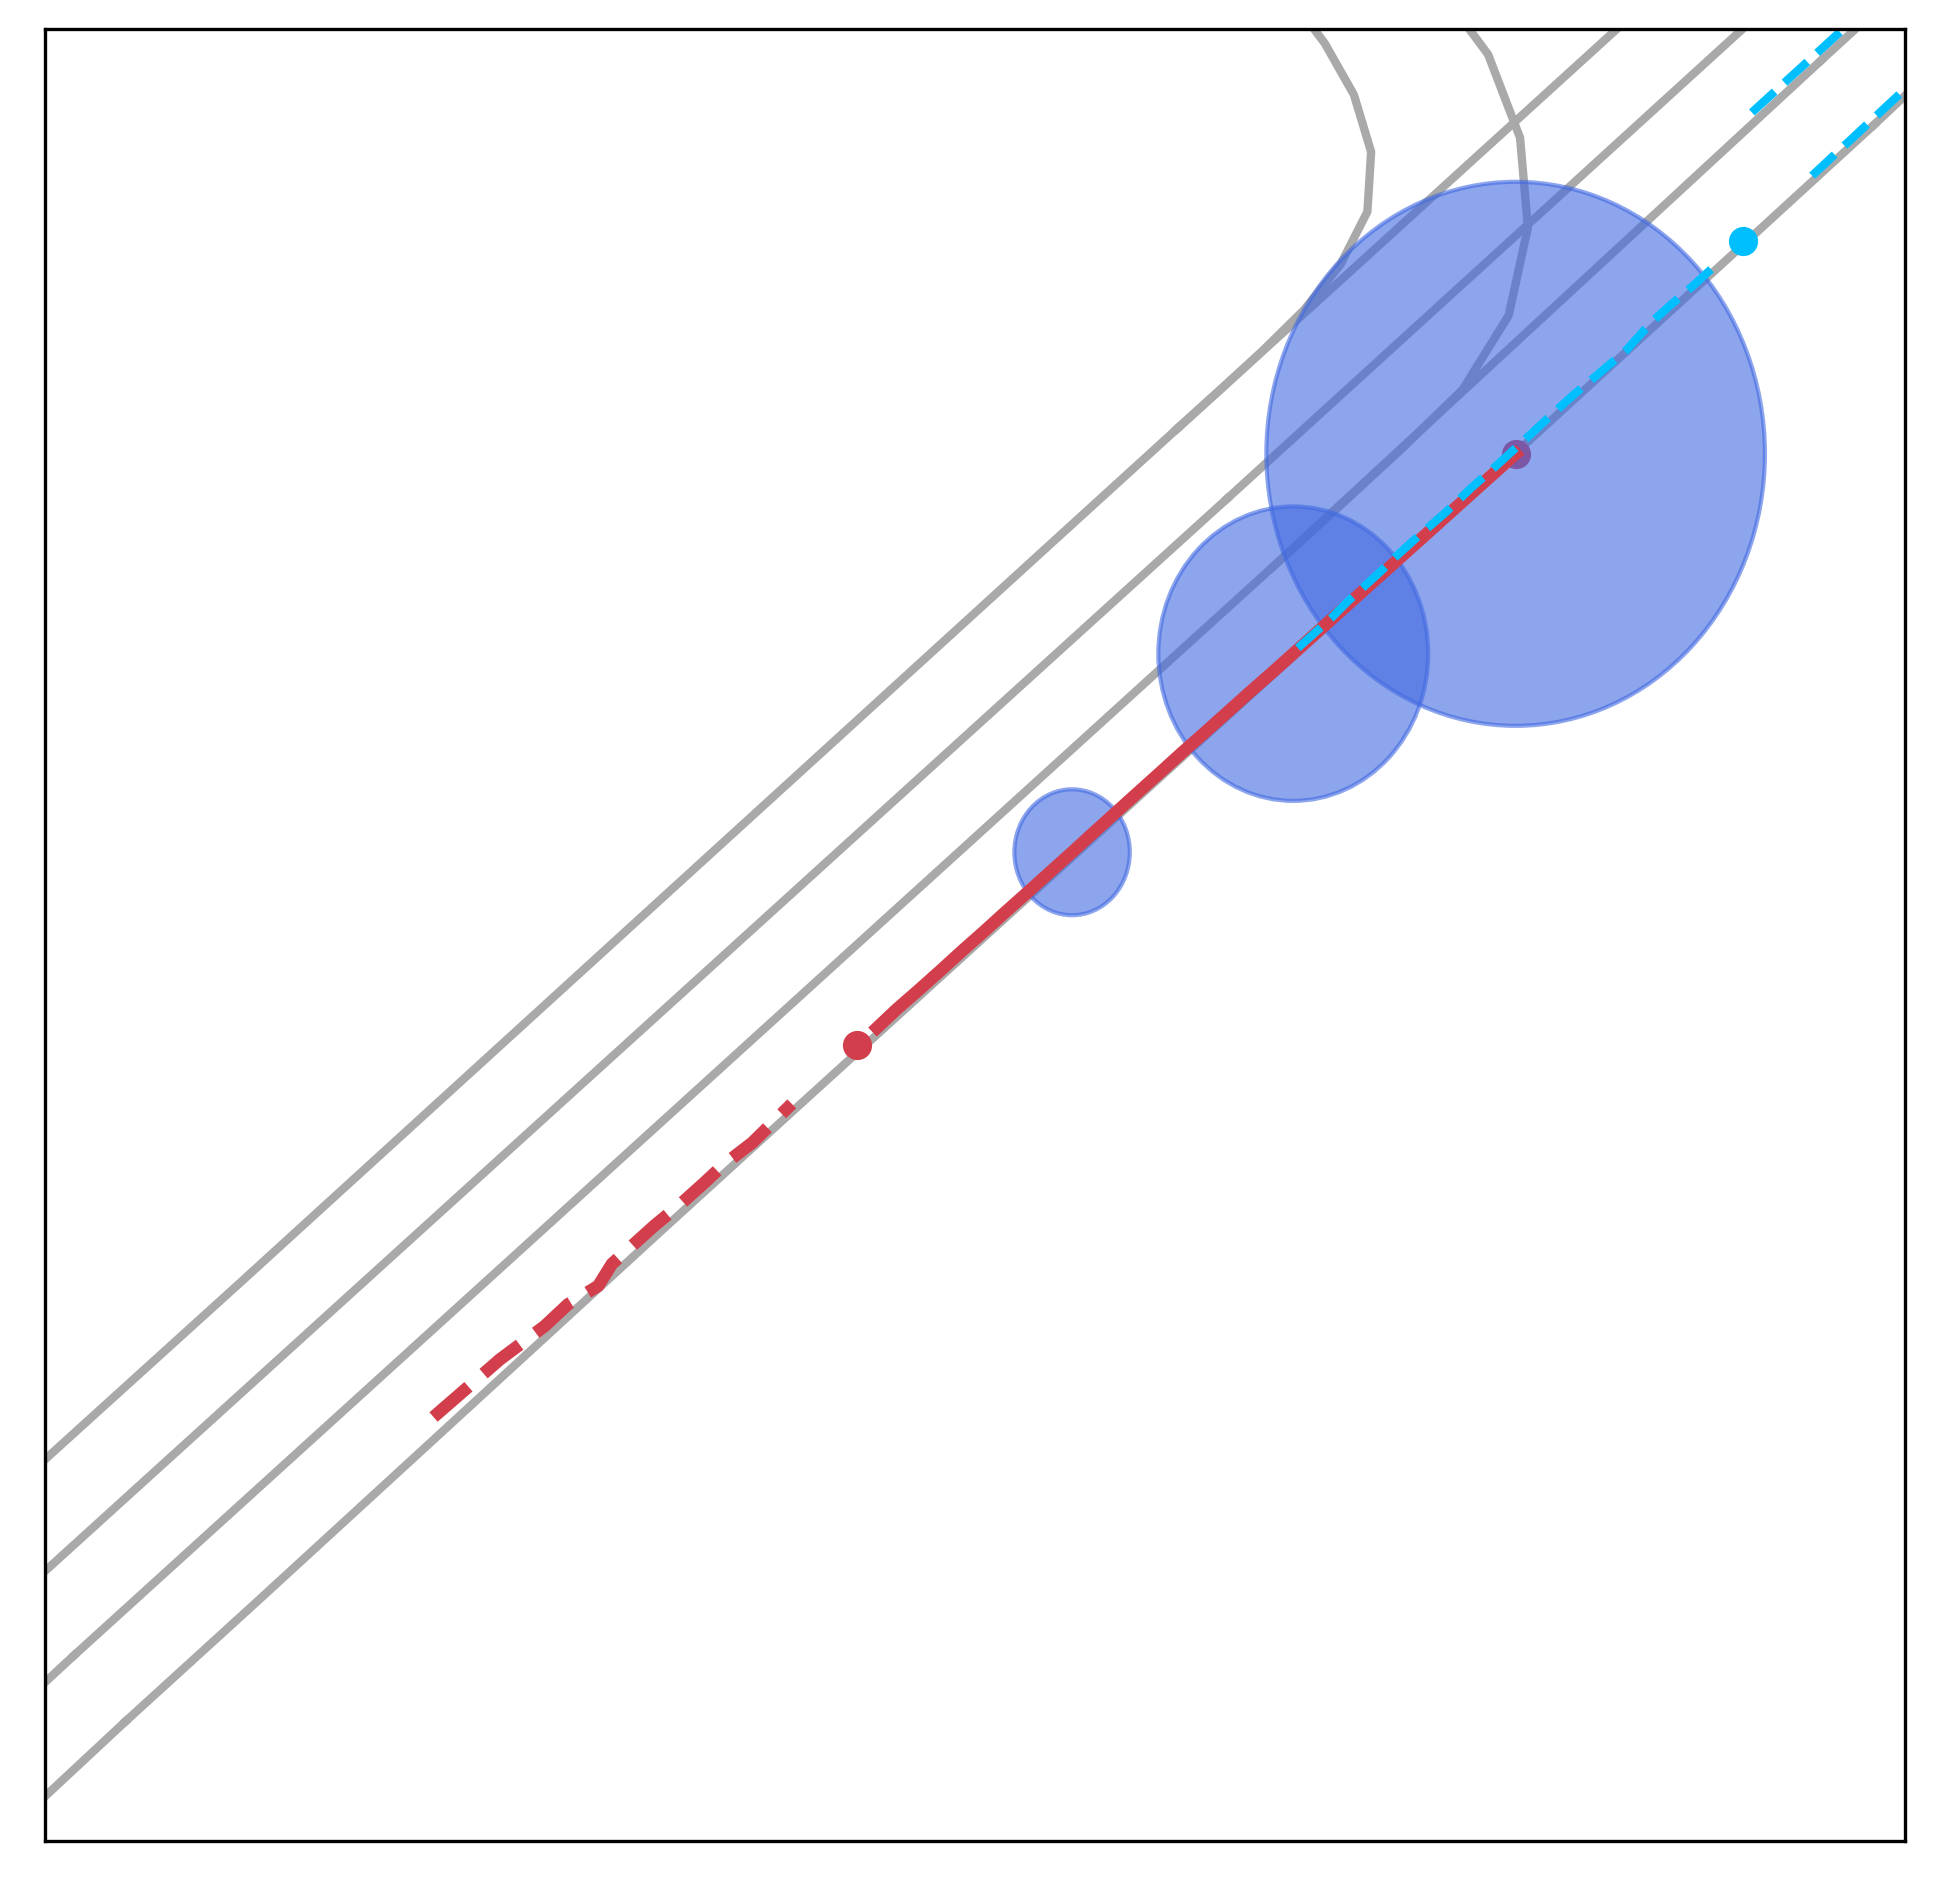
\includegraphics[width=\linewidth]{equivariance/figs/conf2.png}
        \caption{}
    \end{subfigure}%
    \begin{subfigure}[b]{0.245\linewidth}
        \centering
        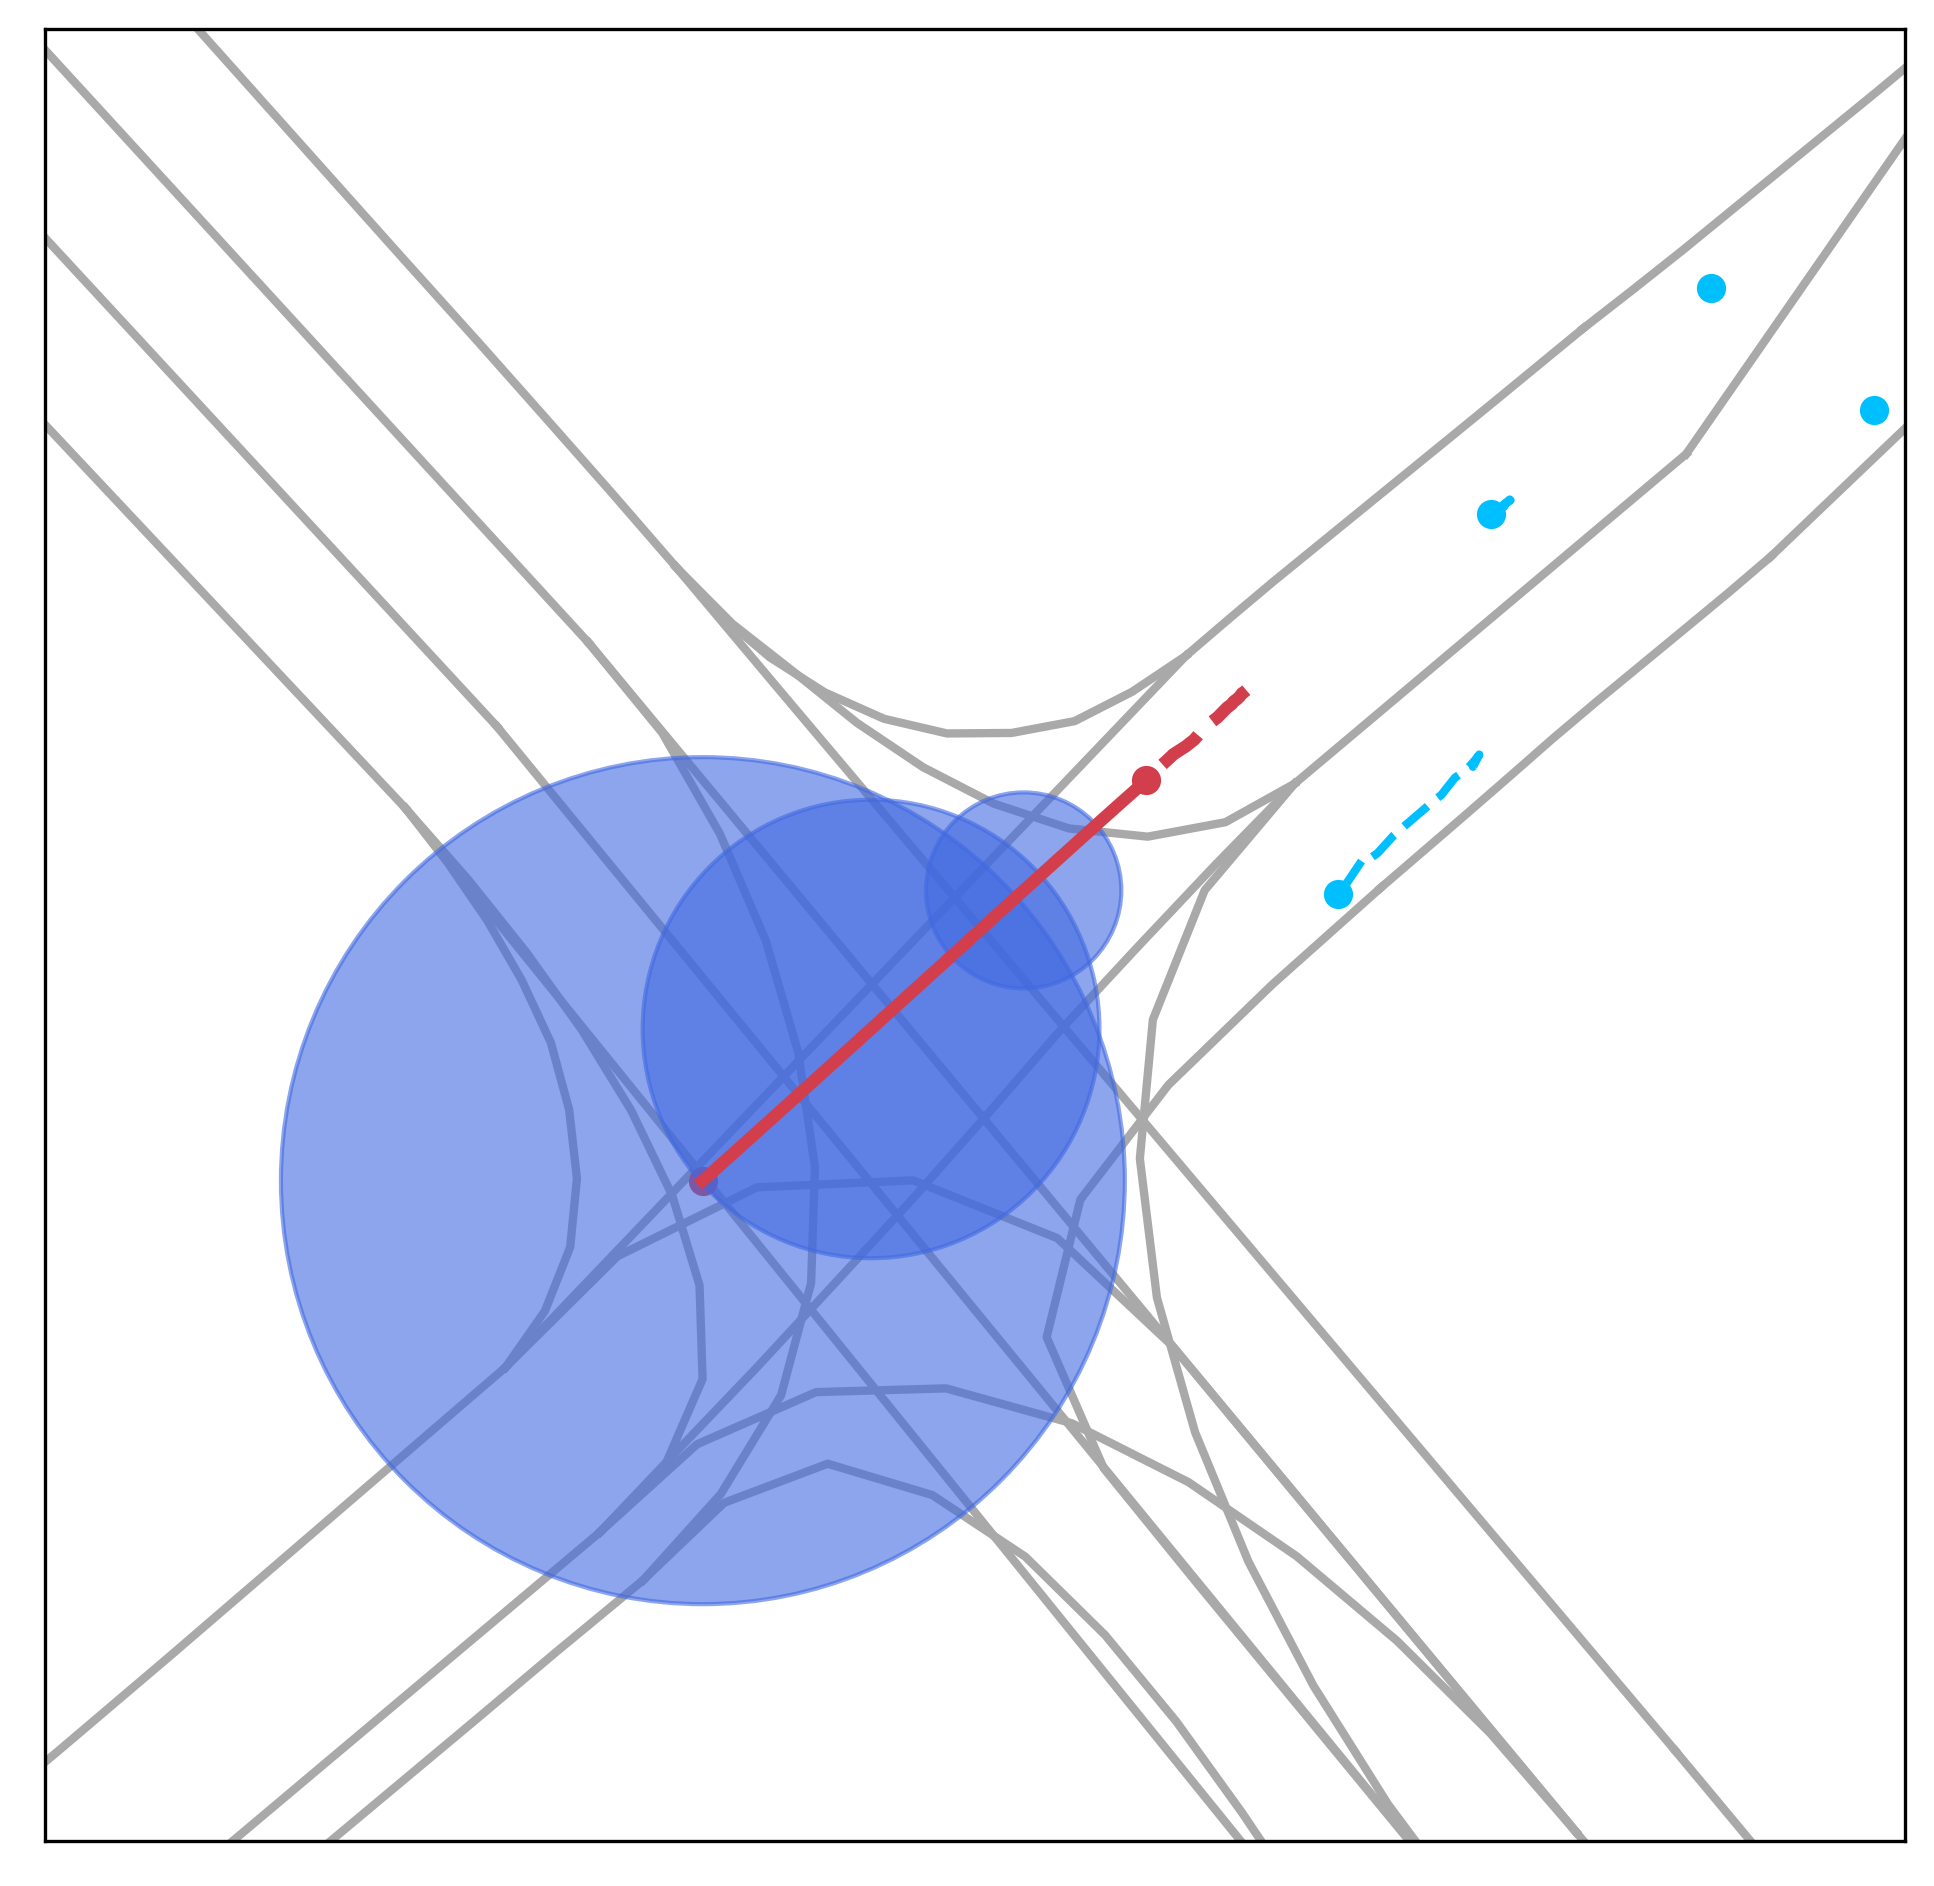
\includegraphics[width=\linewidth]{equivariance/figs/conf3.png}
        \caption{}
        \label{fig:conf3}
    \end{subfigure}%
    \begin{subfigure}[b]{0.245\linewidth}
        \centering
        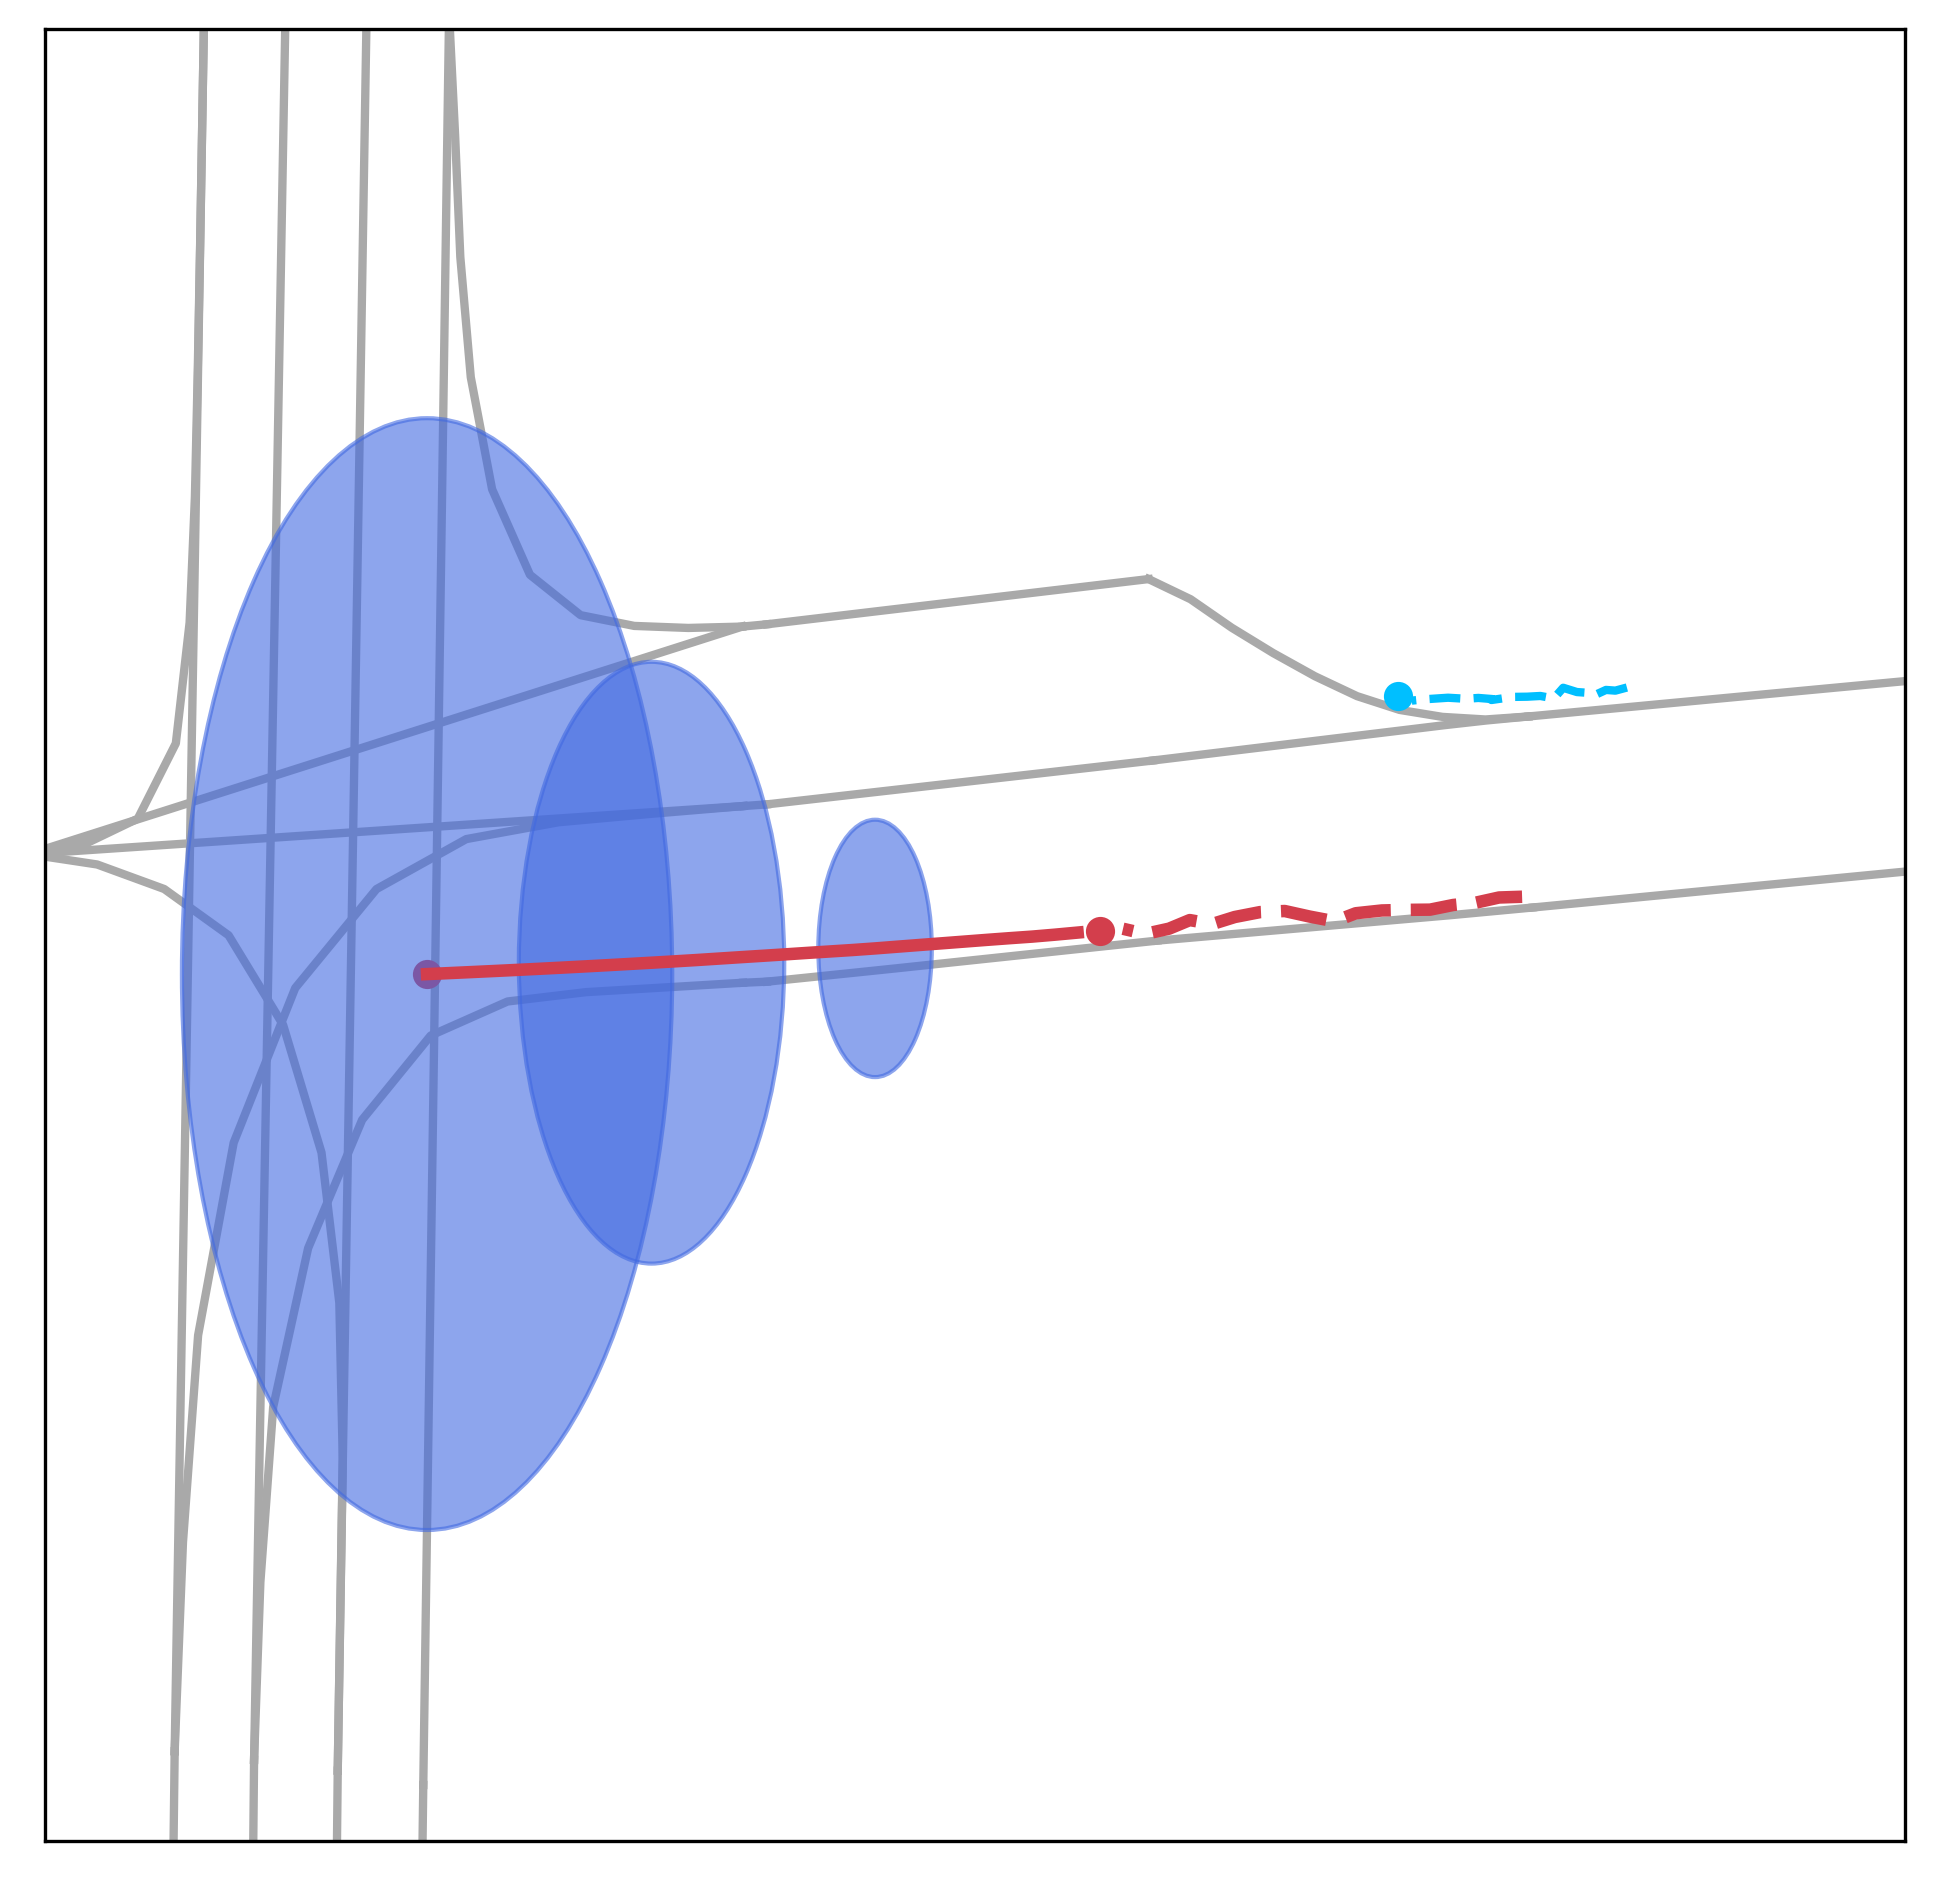
\includegraphics[width=\linewidth]{equivariance/figs/conf7.png}
        \caption{}
        \label{fig:conf7}
    \end{subfigure}
    \caption{Scene illustrations for confidence regions given by conformal-ECCO. Note that in order to achieve 90\% coverage, the region is larger than needed, especially in straight-lane cases like left two scenarios. Due to the lack of underlying assumption about the distribution, the model isn't able to adjust the shape of uncertainty according to data either.}
    \label{fig:conformal}
\end{figure*}


\section{Supplementary: Experiment Details}

\subsection{Implementation Details}
\label{app:exp}

The numbers  in \autoref{tab:big-table} are reported on the official validation set for Argoverse, and on a 10\% test split for TrajNet++. For the particle dataset, the reported numbers are also on a 10\% test split.

\paragraph{Dataset and Preprocessing} 
The synthetic particle dataset is generated by the spring dynamics simulator in \cite{nri}. We added $\sigma=0.01$ noise to the dynamics each step to introduce some uncertainty. The dataset consists of 12,000 time series of trajectories of 5 interacting particles over 50 timesteps ; we use 30 steps as input and predict the following 20 steps. 1,000 samples are used for model validation and 1,000 are used for testing.

The Argoverse autonomous vehicle dataset contains 205,942 samples, consisting of diverse driving scenarios from Miami and Pittsburgh.  We split 90/10 into a training set and validation set of size 185,348 and 20,594 respectively. The official validation set of size 39,472 is used for testing and reporting performance. We preprocess the scenes to filter out incomplete trajectories and cap the number of vehicles modeled to 60. If there are less than 60 cars in the scenario, we insert dummy cars into them to achieve consistent car numbers. For map information, we only include center lanes with lane directions as features. Similar to vehicles, we introduce dummy lane nodes into each scene to make lane numbers consistently equal to 650.

We use the latest release of the TrajNet++ dataset (Update 4.0) for our pedestrian experiments. TrajNet++ is a compiled set of pedestrian trajectories captured in both
indoor and outdoor locations such as in universities, hotels, Zara, and train stations. The sample in this dataset is 21 timestamps long, and the goal is to predict the 2D spatial positions for each pedestrian in the future 12 timestamps given the first 9.
The pedestrian dataset contains 240,896 samples, which we split 80/10/10 into train, validation, and test sets. Similar to Argoverse, we filter out incomplete trajectories in processing and either cap or insert dummy pedestrians such that each scene has 60 agents. No map information was used in the pedestrian dataset. 

We include our code for preprocessing, model implementation, and training in the supplementary materials.

\paragraph{Hyperparameters and Training Details} We trained the PECCO model with 4 equivariant continuous convolution layers of hidden size of (8, 16, 16, 16) respectively for Argoverse, and (4, 8, 16, 16) for the Trajnet++ pedestrian dataset. Our models are all trained with Adam optimizer with a base learning rate $r = 0.001$, and linear learning rate scheduler set to $\gamma = 0.95$.  For Argoverse task, we set the CtsConv radius to be 40, and for the pedestrian task we set it to be 6. PECCO's Arogoverse model has 129k parameters. For comparison, Trajectron++ has 127k and MFP has 67K. 

All our models without map information are trained for 10K iterations with batch size 32 with learning rate updating every 150 iterations. Most of our experiments are performed on a server with 4 RTX 2080 Ti GPUs, and it takes around 9-12 hours to finish training. We run each experiment 3 times with different random initialization and data order. The numbers reported in tables \ref{tab:big-table}, \ref{tab:conformal}, and \ref{tab:deterministic} are the mean and standard deviation of those 3 runs. 

\subsection{Deterministic Baseline Results}
\label{app:deterministic}
We present numbers for deterministic baseline models for Argoverse and Trajnet++. By sampling, we achieve better minADE/minFDE performance with probabilistic models, but they serve as valuable baselines to illustrate the difficulty of the task. 
\begin{table*}[h]
\centering
\begin{tabular}{ c| c c | c c  } 
 \toprule
   &  \multicolumn{2}{c}{Argoverse}  & \multicolumn{2}{c}{Trajnet++}  \\ 
  \midrule
  \textbf{Model}  &  ADE$ \downarrow$ & FDE$\downarrow$ & ADE$ \downarrow$ & FDE$\downarrow$ \\ 
  \midrule
Constant Velocity & 2.77 & 6.16 &1.21 & 2.37\\
Nearest Neighbor   & 3.52 & 7.85 & 1.25 & 2.61\\
LSTM    & 1.97 \plusminus{.05} & 4.98 \plusminus{.31} &1.01  \plusminus{.02}  & 1.98  \plusminus{.08} \\
CtsConv & 1.87 \plusminus{.06} & 4.43 \plusminus{.28} &1.35  \plusminus{.05} & 2.97 \plusminus{.16} \\
ECCO    & 1.68 \plusminus{.04} & 3.98 \plusminus{.19}  & 0.94  \plusminus{.01}  & 2.05 \plusminus{.03} \\
\bottomrule
\end{tabular}
\caption{ Deterministic baselines on the Argoverse and TrajNet++ dataset}
\label{tab:deterministic}
\end{table*}



% \subsection{Visualizations}
% We include 3 more scenarios for qualitatively comparison between models. They provide insights consistent with \autoref{fig:arg-experiment}: LSTM-MRS-r tends to overestimate uncertainty while CtsConv models tend to underestimate collapsing into one mode. PECCO, on the other hand, forecasts a tighter probability that covers the possibilities well.
% \begin{figure*}[ht]
% \centering
% \begin{subfigure}
%   \centering
%   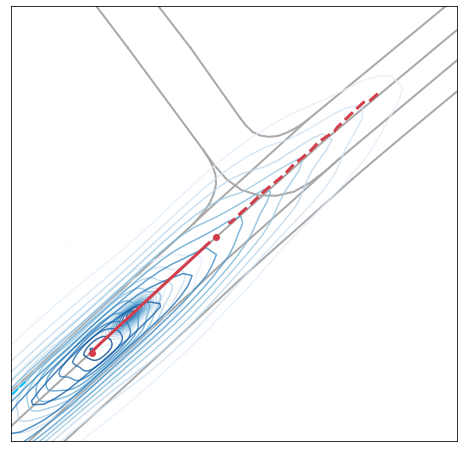
\includegraphics[width=.245\linewidth]{equivariance/figs/10011lstm.png}
%   \caption{LSTM-MRS-r}
%   \label{fig:sub1}
% \end{subfigure}%
% \begin{subfigure}
%   \centering
%   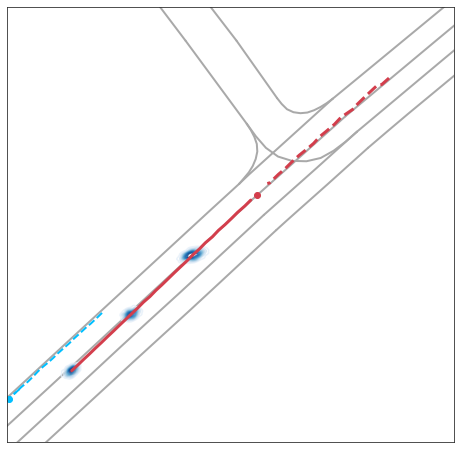
\includegraphics[width=.245\linewidth]{equivariance/figs/10011nll.png}
%   \caption{CtsConv-NLL}
%   \label{fig:sub2}
% \end{subfigure}
% \begin{subfigure}
%   \centering
%   \includegraphics[width=.245\linewidth]{equivariance/figs/10011mis.png}
%   \caption{CtsConv-MRS}
%   \label{fig:sub3}
% \end{subfigure}%
% \begin{subfigure}
%   \centering
%   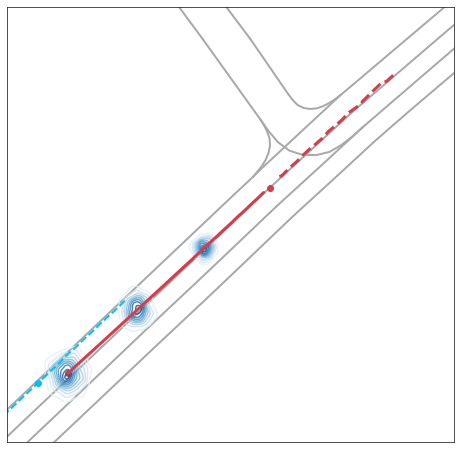
\includegraphics[width=.24\linewidth]{equivariance/figs/10011dyna.png}
%   \caption{PECCO}
%   \label{fig:sub4}
% \end{subfigure}
% \caption{Another lane change example. Red trajectories is the agent of interest in the same scenario. CtsConv-NLL and CtsConv-MRS captured two different modes of futures, whereas PECCO is able to cover both.}
% \label{fig:arg-experiment-2}
% \end{figure*}



% \begin{figure*}[ht]
% \centering
% \begin{minipage}{0.245\textwidth}
%   \centering
%   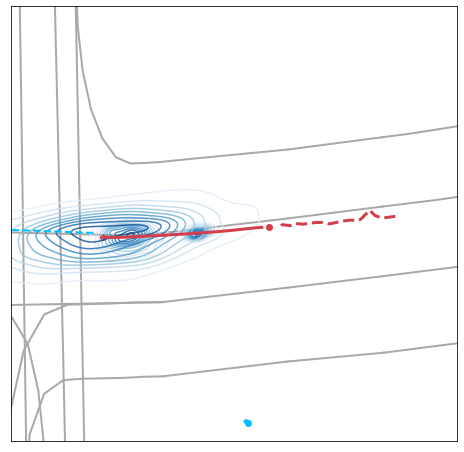
\includegraphics[width=.9\linewidth]{equivariance/figs/10057lstm.png}
%   \subcaption{LSTM-MRS-r}
%   \label{fig:sub1}
% \end{minipage}%
% \begin{minipage}{0.245\textwidth}
%   \centering
%   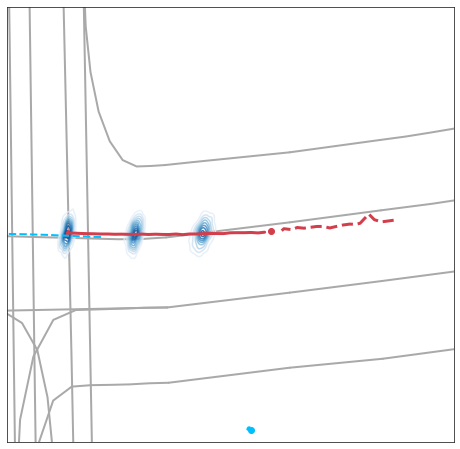
\includegraphics[width=.9\linewidth]{equivariance/figs/10057nll.png}
%   \subcaption{CtsCov-NLL}
%   \label{fig:sub2}
% \end{minipage}%
% \begin{minipage}{0.245\textwidth}
%   \centering
%   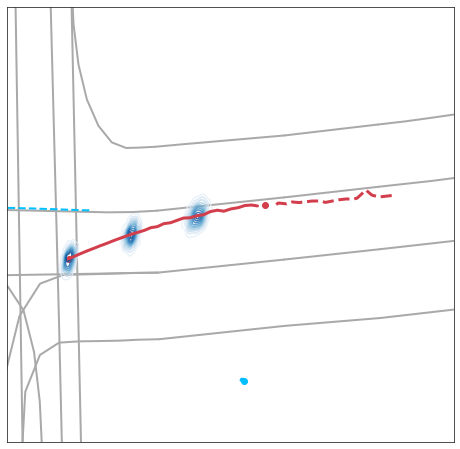
\includegraphics[width=.9\linewidth]{equivariance/figs/10057mis.png}
%   \subcaption{CtsConv-MRS}
%   \label{fig:sub3}
% \end{minipage}%
% \begin{subfigure}
%   \centering
%   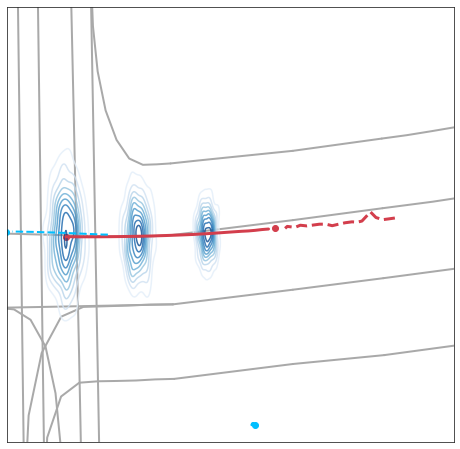
\includegraphics[width=.23\linewidth]{equivariance/figs/10057dyna.png}
%   \caption{PECCO}
%   \label{fig:sub4}
% \end{subfigure}\\
% \begin{subfigure}
%   \centering
%   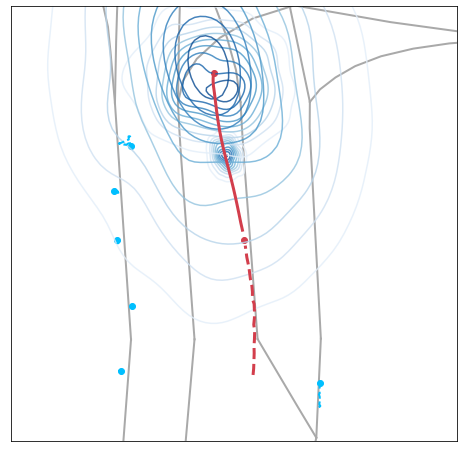
\includegraphics[width=.23\linewidth]{equivariance/figs/10003lstm.png}
%   \caption{LSTM-MRS-r}
%   \label{fig:sub1}
% \end{subfigure}%
% \begin{subfigure}
%   \centering
%   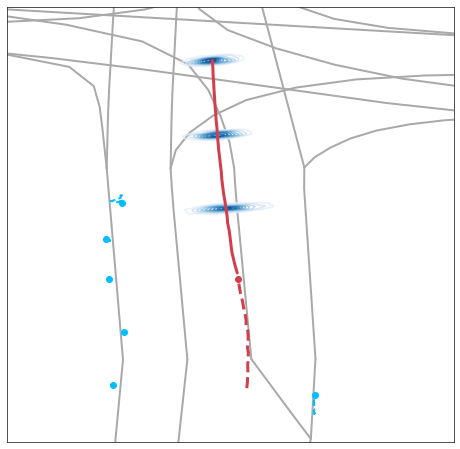
\includegraphics[width=.23\linewidth]{equivariance/figs/10003nll.png}
%   \caption{CtsConv-NLL}
%   \label{fig:sub2}
% \end{subfigure}
% \begin{subfigure}
%   \centering
%   \includegraphics[width=.23\linewidth]{equivariance/figs/10003mis.png}
%   \caption{CtsConv-MRS}
%   \label{fig:sub3}
% \end{subfigure}%
% \begin{subfigure}
%   \centering
%   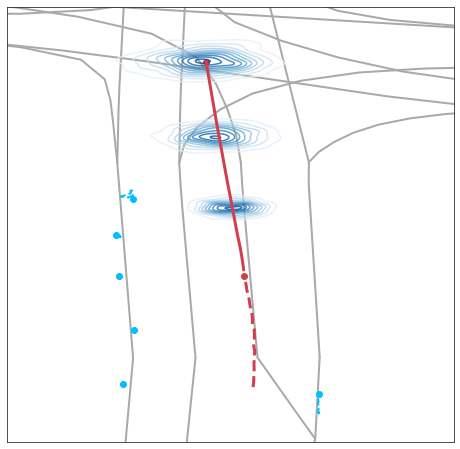
\includegraphics[width=.23\linewidth]{equivariance/figs/10003dyna.png}
%   \caption{PECCO}
%   \label{fig:sub4}
% \end{subfigure}
% \caption{Comparison of uncertainty predicted at 2 crossroads. Red trajectories is the agent of interest in the same scenario. Note how the LSTM predicted uncertainty explodes at the final time step, and PECCO is able to model the possibility of turns. }
% \label{fig:arg-experiment-1}
% \end{figure*}




% %-- archive--

% \begin{figure*}[ht]
% \centering
% \begin{subfigure}
%   \centering
%   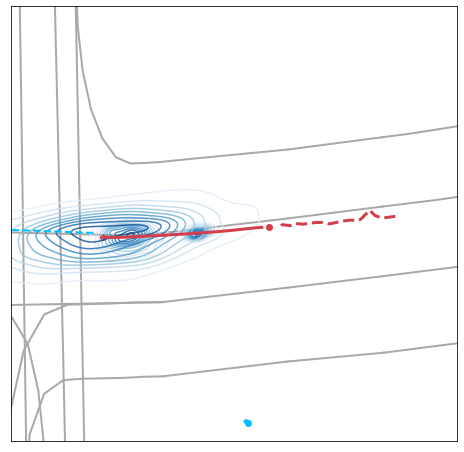
\includegraphics[width=.23\linewidth]{equivariance/figs/10057lstm.png}
%   \caption{LSTM-MRS-r}
%   \label{fig:sub1}
% \end{subfigure}%
% \begin{subfigure}
%   \centering
%   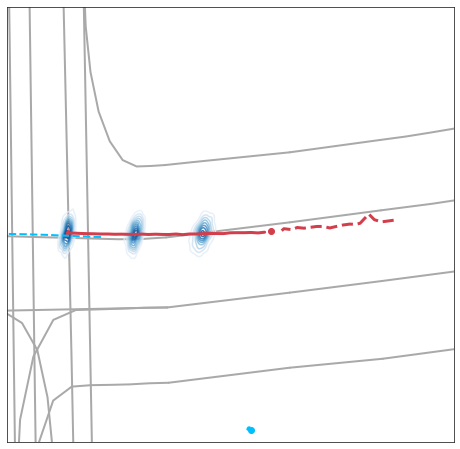
\includegraphics[width=.23\linewidth]{equivariance/figs/10057nll.png}
%   \subcaption{CtsCov-NLL}
%   \label{fig:sub2}
% \end{subfigure}
% \begin{subfigure}
%   \centering
%   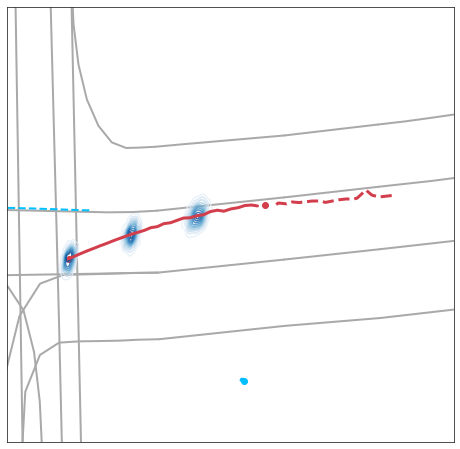
\includegraphics[width=.23\linewidth]{equivariance/figs/10057mis.png}
%   \caption{CtsConv-MRS}
%   \label{fig:sub3}
% \end{subfigure}%
% \begin{subfigure}
%   \centering
%   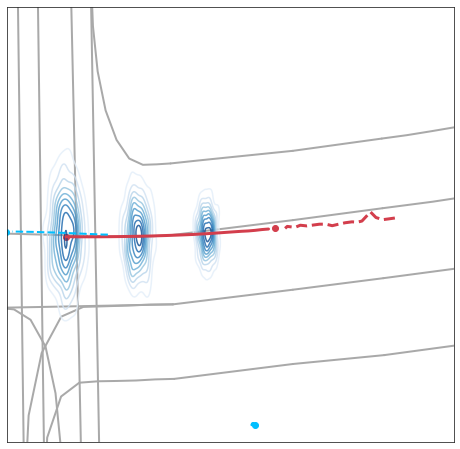
\includegraphics[width=.23\linewidth]{equivariance/figs/10057dyna.png}
%   \caption{PECCO}
%   \label{fig:sub4}
% \end{subfigure}\\
% \begin{subfigure}
%   \centering
%   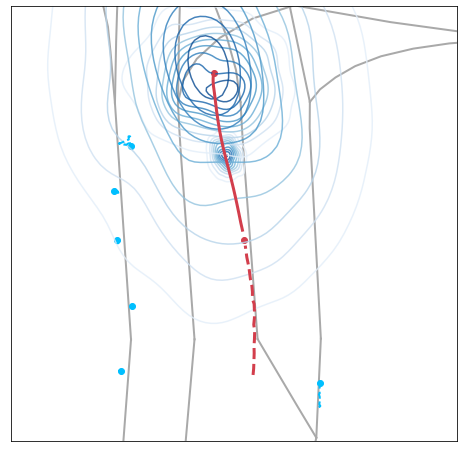
\includegraphics[width=.23\linewidth]{equivariance/figs/10003lstm.png}
%   \caption{LSTM-MRS-r}
%   \label{fig:sub1}
% \end{subfigure}%
% \begin{subfigure}
%   \centering
%   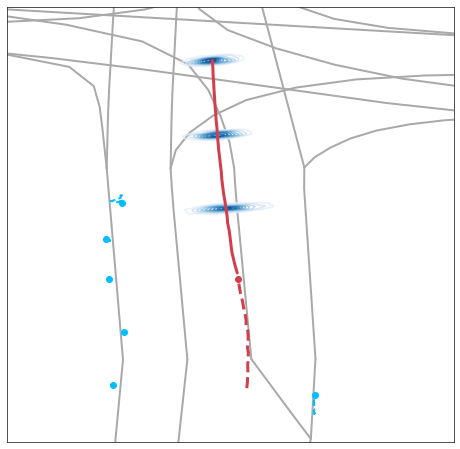
\includegraphics[width=.23\linewidth]{equivariance/figs/10003nll.png}
%   \caption{CtsConv-NLL}
%   \label{fig:sub2}
% \end{subfigure}
% \begin{subfigure}
%   \centering
%   \includegraphics[width=.23\linewidth]{equivariance/figs/10003mis.png}
%   \caption{CtsConv-MRS}
%   \label{fig:sub3}
% \end{subfigure}%
% \begin{subfigure}
%   \centering
%   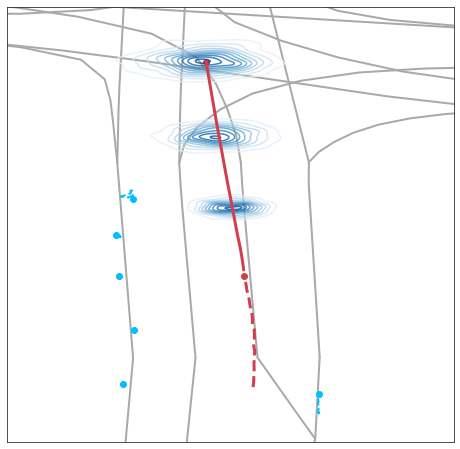
\includegraphics[width=.23\linewidth]{equivariance/figs/10003dyna.png}
%   \caption{PECCO}
%   \label{fig:sub4}
% \end{subfigure}
% \caption{Comparison of uncertainty predicted at 2 crossroads. Red trajectories is the agent of interest in the same scenario. Note how the LSTM predicted uncertainty explodes at the final time step, and PECCO is able to model the possibility of turns. }
% \label{fig:arg-experiment-1}
% \end{figure*}




%\textbf{Model Parameters and Data Efficiency.}
%A major benefit of incorporating the inductive bias of equivariance is to improve the sample efficiency of learning, as equivariance collapses the domain space by a factor of the size of the symmetry group \cite{wang2020incorporating}. Thus PECCO requires far fewer samples to learn from.
